%% POSIM - ESWA Journal Submission
\documentclass[a4paper,fleqn]{cas-dc}

\usepackage[authoryear,longnamesfirst]{natbib}
\usepackage{amsmath}
\usepackage{algorithm}
\usepackage{algorithmic}
\usepackage{array}
\usepackage{graphicx}
\usepackage{booktabs}
\usepackage{multirow}
\usepackage{colortbl}
\usepackage{xcolor}
\usepackage{makecell}
\usepackage[most]{tcolorbox}
\usepackage{subfig}
\usepackage{wrapfig}
\usepackage{fontspec}
\setmainfont{Times New Roman}
\setsansfont{Arial}
\setmonofont{Courier New}
\ExplSyntaxOn
\cs_if_exist:cT { not= } { \cs_undefine:c { not= } }
\cs_if_exist:cT { not< } { \cs_undefine:c { not< } }
\cs_if_exist:cT { not> } { \cs_undefine:c { not> } }
\ExplSyntaxOff
\usepackage{unicode-math}
\setmathfont{XITS Math}

\usepackage{listings}
\lstset{
  basicstyle=\scriptsize\ttfamily,
  breaklines=true,
  frame=none,
  columns=fullflexible,
  keepspaces=true,
  aboveskip=2pt,
  belowskip=2pt,
}
\usepackage{etoolbox}
\usepackage{placeins}
\AtBeginEnvironment{tabular}{\fontspec{Times New Roman}}

\renewcommand{\footnotesize}{\scriptsize}

\usepackage{caption}
\captionsetup{font={small,rm},labelfont={bf},labelsep=newline}
\captionsetup[table]{font={small,rm},labelfont={bf},labelsep=newline}
\captionsetup[figure]{font={small,rm},labelfont={bf},labelsep=newline}

\hypersetup{citecolor={blue!80!black},linkcolor={blue!80!black},urlcolor={blue!80!black}}
\graphicspath{{figures/}}

\definecolor{oursrow}{RGB}{232,245,233}
\definecolor{greenrow}{RGB}{228,245,228}
\definecolor{orangerow}{RGB}{255,245,230}
\definecolor{purplerow}{RGB}{245,240,255}
\definecolor{grayrow}{RGB}{240,240,240}
\definecolor{promptbg}{RGB}{242,247,253}
\definecolor{promptborder}{RGB}{70,130,180}
\definecolor{gaingreen}{RGB}{34,139,34}

\newtcolorbox{promptbox}{
 colback=promptbg, colframe=promptborder,
 boxrule=0.5pt, arc=1mm,
 left=4pt, right=4pt, top=4pt, bottom=4pt,
 breakable, enhanced}

\newcommand{\best}[1]{\textbf{#1}}
\newcommand{\na}{\text{---}}
\newcommand{\posim}{\textsc{Posim}}
\newcommand{\gain}[1]{{\textcolor{gaingreen}{\,#1}}}

\def\tsc#1{\csdef{#1}{\textsc{\lowercase{#1}}\xspace}}
\tsc{WGM}
\tsc{QE}

\begin{document}
\let\WriteBookmarks\relax
\def\floatpagepagefraction{1}
\def\textpagefraction{.001}

\shorttitle{POSIM: A Multi-Agent Framework for Social Media Public Opinion Simulation}
\shortauthors{Y. Zhang et al.}

\title [mode = title]{POSIM: A Multi-Agent Simulation Framework for Social Media Public Opinion Evolution}

\author{Yongmao Zhang}
\credit{Conceptualization, Methodology, Software, Writing - Original draft}

\author{Kai Qiao}

\author{Zhengyan Wang}

\author{Wenyao Sun}

\author{Dekui Ma}

\author{Ningning Liang}

\author{Jian Chen}

\author{Bin Yan}
\cormark[1]

\affiliation{organization={Henan Key Laboratory of Imaging and Intelligent Processing, Information Engineering University},
            city={Zhengzhou},
            postcode={450001},
            country={PR China}}

\cortext[1]{Corresponding author}
\fntext[1]{These authors contributed equally to this work.}

\begin{abstract}
The evolution of public opinion on social media profoundly shapes governance decisions, making its reliable modeling and anticipation critically important. Traditional approaches, including epidemic models and rule-based agent-based models (ABMs), struggle to capture the complex cognitive processes and adaptive behaviors of real social media users. Recent advances in large language model (LLM)-based social simulation have been applied to analyze polarization, conformity, and information cascading, yet they still fall short of reproducing the irrational individual interactions and multi-phase dynamics that characterize real-world public opinion events.
This paper introduces POSIM (\textbf{P}ublic \textbf{O}pinion \textbf{Sim}ulator), a multi-agent simulation framework for social media public opinion evolution. POSIM constructs LLM-powered agents whose cognitive architecture draws on Belief-Desire-Intention (BDI) theory to simulate cognitively grounded social media users, builds a virtual social media environment with social networks and content exposure mechanisms, and incorporates a Hawkes point process-based temporal dynamics engine that captures the multi-phase co-evolution between agents and their environment.
To rigorously assess the framework's credibility, we collect real-world public opinion datasets from the Weibo platform covering the full interaction chain of original posts, reposts, and comments. Experiments show that POSIM successfully reproduces key characteristics of real public opinion at both the micro-level interaction mechanisms and macro-level emergent phenomena, with effectiveness confirmed across multiple quantitative metrics. We further conduct governance-oriented intervention experiments and uncover findings of considerable theoretical and practical value, including an ``empathy paradox.'' These results demonstrate that POSIM can serve as a computational experiment platform for effective ex-ante strategy evaluation, providing quantifiable decision support for public opinion governance.
\end{abstract}

\begin{keywords}
Social media simulation \sep Public opinion analysis \sep Large language model \sep Agent cognitive architecture \sep Hawkes process
\end{keywords}

\maketitle

% ============================================================
% Section 1: Introduction
% ============================================================
\section{Introduction}\label{sec:intro}

Social media has become a pivotal arena for the formation, fermentation, and spread of public opinion. A single breaking event can trigger massive user participation within hours, accompanied by complex collective emotional arousal~\citep{gonzalez_emotional_2010} and information cascades~\citep{goldstein_structure_2012}. Understanding and anticipating how public opinion evolves is therefore of substantial importance to social governance~\citep{WU2025127823}. Real-world social experiments, however, are fundamentally constrained by ethical concerns, irreproducibility, and uncontrollable variables, making it impractical to repeatedly test different mechanisms and intervention strategies in realistic settings. Computational simulation consequently serves as a vital technical pathway for studying opinion evolution dynamics, conducting strategy evaluation, and informing governance decisions~\citep{bonabeau_agent-based_2002}.

Building a simulation system that faithfully replicates real public opinion evolution is far from straightforward. On the one hand, social media user behavior is not the product of simple rational calculation but is shaped by the interplay of individual cognition and environmental factors~\citep{buckels2014trolls}, requiring the system to model this complex cognitive decision process. On the other hand, opinion dynamics exhibit pronounced temporal characteristics: events often erupt intensely within short periods and undergo multi-phase evolution involving outbreak, decline, and resurgence~\citep{ZHOU2024121307}, imposing stringent demands on the temporal precision of simulation~\citep{zhao_seismic_2015}. Any simulation system must also address a fundamental credibility question: it should not only produce outputs that approximate real data, but also demonstrate that its internal mechanisms are reasonable and interpretable~\citep{mcculloch_calibrating_2022}. Traditional opinion modeling approaches such as epidemic models~\citep{daley_stochastic_1965} and threshold cascade models~\citep{granovetter_threshold_1978} typically reduce individuals to a handful of discrete states, making it difficult to represent complex semantics, interaction strategies, and user heterogeneity. Agent-based modeling (ABM), while providing a bottom-up simulation paradigm~\citep{macal_tutorial_2010} often combined with opinion dynamics rules to characterize collective evolution~\citep{castellano_statistical_2009}, still relies on rule-driven agents that cannot capture the cognitive reasoning, nuanced interactions, and platform-coupling processes of real users.

In recent years, large language model (LLM)-driven social simulation has brought fresh momentum to this field~\citep{wang_survey_2024}. Generative Agent-Based Modeling (GABM), exemplified by generative agents~\citep{park_generative_2023}, demonstrates that LLM agents can produce human-like social behaviors and give rise to complex phenomena such as polarization, conformity, and information diffusion through multi-agent interaction~\citep{gao_s3_2023,chuang_simulating_2024}. To model the more intricate evolution of real public opinion events, however, it is necessary to further capture the non-rational characteristics of users driven by cognitive beliefs, and to reproduce the co-evolutionary process from environmental triggers through user responses to propagation amplification, all within compressed timeframes. A unified simulation framework that both targets real public opinion evolution and ensures result credibility therefore remains an open challenge.

Against this backdrop, we propose POSIM (\textbf{P}ublic \textbf{O}pinion \textbf{Sim}ulator), a multi-agent simulation framework for real-world social media public opinion evolution. The framework constructs LLM-powered agents inspired by Belief-Desire-Intention (BDI) cognitive theory~\citep{bratman_intention_1987,rao_bdi_1995}, integrating emotional arousal and cognitive biases into a hierarchical cognitive architecture so that each agent possesses explicit cognitive states and a traceable multi-stage decision pipeline. It then builds a virtual social media environment with social networks and content exposure mechanisms, and incorporates a temporal dynamics engine based on the Hawkes self-exciting point process~\citep{hawkes_spectra_1971}, which unifies exogenous event shocks and endogenous user interactions to model multi-phase opinion evolution.

To prevent simulation evaluation from falling into the trap of illusory success, where outputs superficially match real data while the underlying mechanisms remain unexplained, we design a three-layer progressive credibility validation following the ``mechanism--phenomenon--data'' hierarchy~\citep{sargent_verification_2013}, addressing three questions: (1) Are the internal mechanisms sound? (2) Are the emergent group phenomena plausible? (3) Are the simulation outputs statistically reliable? We collect three real-world public opinion datasets from the Weibo platform covering the full interaction chain of original posts, reposts, and comments, and conduct systematic experiments. Results show that POSIM validates the soundness of agent behavioral logic at the mechanism level, exhibits emergent group phenomena consistent with social science theories at the phenomenon level, and achieves effective alignment between simulated outputs and real opinion data at the data level. Governance-oriented intervention experiments based on POSIM further reveal that certain ostensibly positive guidance strategies can produce adverse effects in complex opinion interactions, a counter-intuitive finding that provides important empirical evidence for the design of real-world governance strategies. The main contributions of this work are as follows.

First, we propose POSIM, a multi-agent simulation framework targeting real-world social media public opinion evolution, advancing the modeling objective from general social phenomena simulation toward credible event-specific simulation and governance-oriented strategy evaluation. Second, at the technical level, the framework employs a hierarchical cognitive architecture inspired by BDI theory to model non-rational user decision-making, constructs a virtual environment integrating social networks and content exposure mechanisms to drive multi-agent interaction, and introduces a Hawkes point process temporal engine that jointly models the co-evolution of exogenous event shocks and endogenous user responses. Third, we systematically validate the framework's credibility on three real Weibo public opinion datasets from the mechanism, phenomenon, and data perspectives; governance-oriented intervention experiments further reveal an ``empathy paradox,'' where empathy-based guidance intended to mitigate group conflict instead intensifies negative emotions under complex interactions, providing important empirical evidence for public opinion governance strategy design.

% ============================================================
% Section 2: Related Work
% ============================================================
\section{Related Work}\label{sec:related}

\subsection{Public Opinion Propagation Modeling}
Public opinion propagation modeling aims to characterize the dynamics by which information spreads and evolves across social networks. Early research largely followed epidemic modeling, with the stochastic rumor propagation model~\citep{daley_stochastic_1965} partitioning individuals into ignorant, spreader, and stifler states. Subsequent studies introduced complex network topologies~\citep{watts_strogatz_1998,barabasi_albert_1999} and multi-stage transition mechanisms~\citep{jiang_weibo_spnr_2020} to analyze the influence of network structure on cascade size, while threshold cascade models~\citep{granovetter_threshold_1978,watts_cascades_2002} explained the emergence of collective behavior from the perspective of individual decision thresholds. Beyond the network science perspective, system dynamics~\citep{forrester_industrial_1961,sterman_business_2000} uses stock-flow diagrams and feedback loops to model causal relationships among propagation entities~\citep{gao_sd_public_opinion_2019,liu_evolution_2024}, offering a macro-level view of how system variables shape opinion trajectories, though it treats populations as continuous aggregate flows rather than heterogeneous individuals. On the temporal dynamics front, self-exciting point processes~\citep{hawkes_spectra_1971} and their extensions provide continuous-time parametric tools for social media cascading phenomena, achieving notable success in popularity prediction, yet their focus remains at the population level, with limited capacity for representing individual cognitive processes. In summary, these approaches each have strengths in predicting collective trends but share a common inability to explicitly model individual cognition, a limitation that has increasingly motivated researchers to turn to agent-based modeling paradigms.

\subsection{Agent-Based Modeling and Opinion Dynamics}

Agent-based modeling (ABM) endows large populations of heterogeneous individuals with local behavioral rules and observes emergent collective phenomena, serving as the core paradigm for bottom-up study of social systems~\citep{bonabeau_agent-based_2002,macal_tutorial_2010}. The ODD protocol~\citep{grimm_odd_2010} and parameter calibration methods~\citep{mcculloch_calibrating_2022} further provide standardized procedures for reproducible modeling and systematic validation. This paradigm has yielded substantial results in opinion dynamics: the DeGroot consensus model~\citep{degroot_reaching_1974} describes opinion convergence through weighted averaging, the Deffuant-Weisbuch model~\citep{deffuant_mixing_2000} introduces pairwise interactions to capture local persuasion, and the Hegselmann-Krause bounded confidence model~\citep{hegselmann_opinion_2002} explains group fragmentation through selective exposure. Collectively, these works systematically reproduce phase transitions from consensus to polarization~\citep{castellano_statistical_2009,bernardo_bc_survey_2024}. Building on this foundation, researchers have constructed opinion simulation systems with multiple agent types on social networks~\citep{chen_evolution_2025,wu_public_2023} to investigate polarization and echo chamber effects~\citep{liu_agent-based_2024,banisch_agent_2012,cinelli2021echo_ipm}. Despite these advances, the decision logic of ABM agents depends entirely on predefined numerical rules: opinions are reduced to low-dimensional continuous variables and interactions are constrained to weighted averaging or threshold functions. This rule-driven paradigm can neither perceive the rich contextual information present in real opinion environments nor simulate the emotional evolution, motivated reasoning, and autonomous decision-making that characterize real social media users.

\subsection{LLM-Driven Social Simulation}

Artificial intelligence is undergoing a profound shift from perceptual to cognitive intelligence, and the semantic understanding, contextual reasoning, and autonomous decision-making abilities of large language models open possibilities that transcend traditional rule-based paradigms for social simulation~\citep{wang_survey_2024}. The pioneering GABM work on generative agents~\citep{park_generative_2023} first demonstrated the emergent capacities of LLMs in autonomous planning and social interaction. Since then, GABM has been explored in multiple governance-related domains~\citep{QI2026130753,repec:jas:jasssj:2025-107-3}, though a simulation system reliably applicable to complex public opinion governance remains absent. In parallel, simulation research targeting social media opinion dynamics has progressed rapidly. S3~\citep{gao_s3_2023} was among the first to build an LLM-based information propagation framework, validating the feasibility of language model-driven social interaction. SPARK~\citep{zhang_spark_2025} and LLM-AIDSim~\citep{zhang_llm-aidsim_2025,hu_llm-enhanced_2024} further explored emergent patterns in stance evolution and information diffusion, while FDE-LLM~\citep{yao_social_2025} innovatively fused dynamical equations with language models to impose mathematical constraints on opinion trajectories. Regarding scale and efficiency, OASIS~\citep{yang_oasis_2025} pushed the node count to the million level, demonstrating the scalability potential of LLM-driven simulation; HiSim~\citep{mou_unveiling_2024} adopted a hybrid strategy that achieves a favorable balance between computational efficiency and fidelity; TrendSim~\citep{zhang_trendsim_2025} further attempted to simulate the evolution of trending topics. As shown in Table~\ref{tab:comparison}, these efforts mark important progress, yet existing frameworks generally treat LLMs as end-to-end behavioral decision-makers, lacking explicit modeling of complex user cognitive pipelines and thus ill-equipped to capture non-rational behavior. Most existing work targets generic opinion evolution scenarios, whereas real public opinion events involve irrational individual interactions, multi-phase dynamics, and governance-oriented strategy needs that current frameworks cannot adequately support. Most platforms also lack systematic validation logic, having not established a comprehensive verification framework covering mechanism soundness, phenomenological consistency, and data reliability.

To address these limitations, the POSIM framework proposed in this paper undertakes systematic design along three dimensions, agents, environment, and strategy evaluation, aiming to provide an integrated solution for credible simulation and governance decision support.

\begin{table}[!t]
\centering
\caption{Comparison of POSIM with representative public opinion simulation frameworks.}
\label{tab:comparison}
\renewcommand{\arraystretch}{1.0}
\resizebox{\columnwidth}{!}{%
\scriptsize
\begin{tabular}{@{}lcccccccc@{}}
\toprule
\textbf{Platform} &
\makecell{\textbf{Explicit}\\\textbf{Cognitive}\\\textbf{Modeling}} &
\multicolumn{3}{c}{\textbf{Validation Ladder}} &
\makecell{\textbf{Real-Case}\\\textbf{Intervention}} &
\makecell{\textbf{LLM-Based}\\\textbf{Multi-Type}\\\textbf{Agents}} &
\makecell{\textbf{Temporal}\\\textbf{Precision}} &
\makecell{\textbf{Modular}\\\textbf{Design}} \\
\cmidrule(lr){3-5}
 & & \textbf{M} & \textbf{P} & \textbf{D} & & & & \\
\midrule
S3 & $\times$ & $\times$ & $\checkmark$ & $\checkmark$ & $\times$ & $\times$ & $\bigstar\bigstar\bigstar$ & $\bigstar\bigstar\bigstar$ \\
HiSim & $\times$ & $\times$ & $\times$ & $\checkmark$ & $\times$ & $\times$ & $\bigstar\bigstar$ & $\bigstar\bigstar$ \\
GA-S3 & $\times$ & $\times$ & $\times$ & $\checkmark$ & $\times$ & $\checkmark$ & $\bigstar\bigstar\bigstar$ & $\bigstar\bigstar$ \\
SPARK & $\times$ & $\times$ & $\checkmark$ & $\times$ & $\times$ & $\checkmark$ & $\bigstar\bigstar$ & $\bigstar\bigstar$ \\
FDE-LLM & $\times$ & $\times$ & $\times$ & $\checkmark$ & $\times$ & $\times$ & $\bigstar\bigstar$ & $\bigstar\bigstar$ \\
TrendSim & $\times$ & $\checkmark$ & $\times$ & $\times$ & $\times$ & $\checkmark$ & $\bigstar\bigstar\bigstar\bigstar$ & $\bigstar\bigstar\bigstar$ \\
OASIS & $\times$ & $\times$ & $\checkmark$ & $\checkmark$ & $\times$ & $\times$ & $\bigstar\bigstar\bigstar\bigstar$ & $\bigstar\bigstar\bigstar\bigstar$ \\
LMAgent & $\times$ & $\times$ & $\times$ & $\checkmark$ & $\times$ & $\checkmark$ & $\bigstar\bigstar$ & $\bigstar\bigstar$ \\
\midrule
\rowcolor{grayrow}
\textit{\textbf{POSIM (Ours)}} & $\checkmark$ & $\checkmark$ & $\checkmark$ & $\checkmark$ & $\checkmark$ & $\checkmark$ & $\bigstar\bigstar\bigstar\bigstar\bigstar$ & $\bigstar\bigstar\bigstar\bigstar\bigstar$ \\
\bottomrule
\end{tabular}%
}
\par\vspace{2pt}
{\scriptsize\fontspec{Times New Roman}\selectfont
\parbox{\columnwidth}{\raggedright \textit{Note}: $\bigstar$ denotes capability level (1--5); M, P, and D denote mechanism, phenomenon, and data validation; real-case intervention denotes controlled experiments on real-world events.}}
\end{table}

% ============================================================
% Section 3: Method
% ============================================================
\section{Method}\label{sec:method}

\begin{figure*}[!t]
\centering
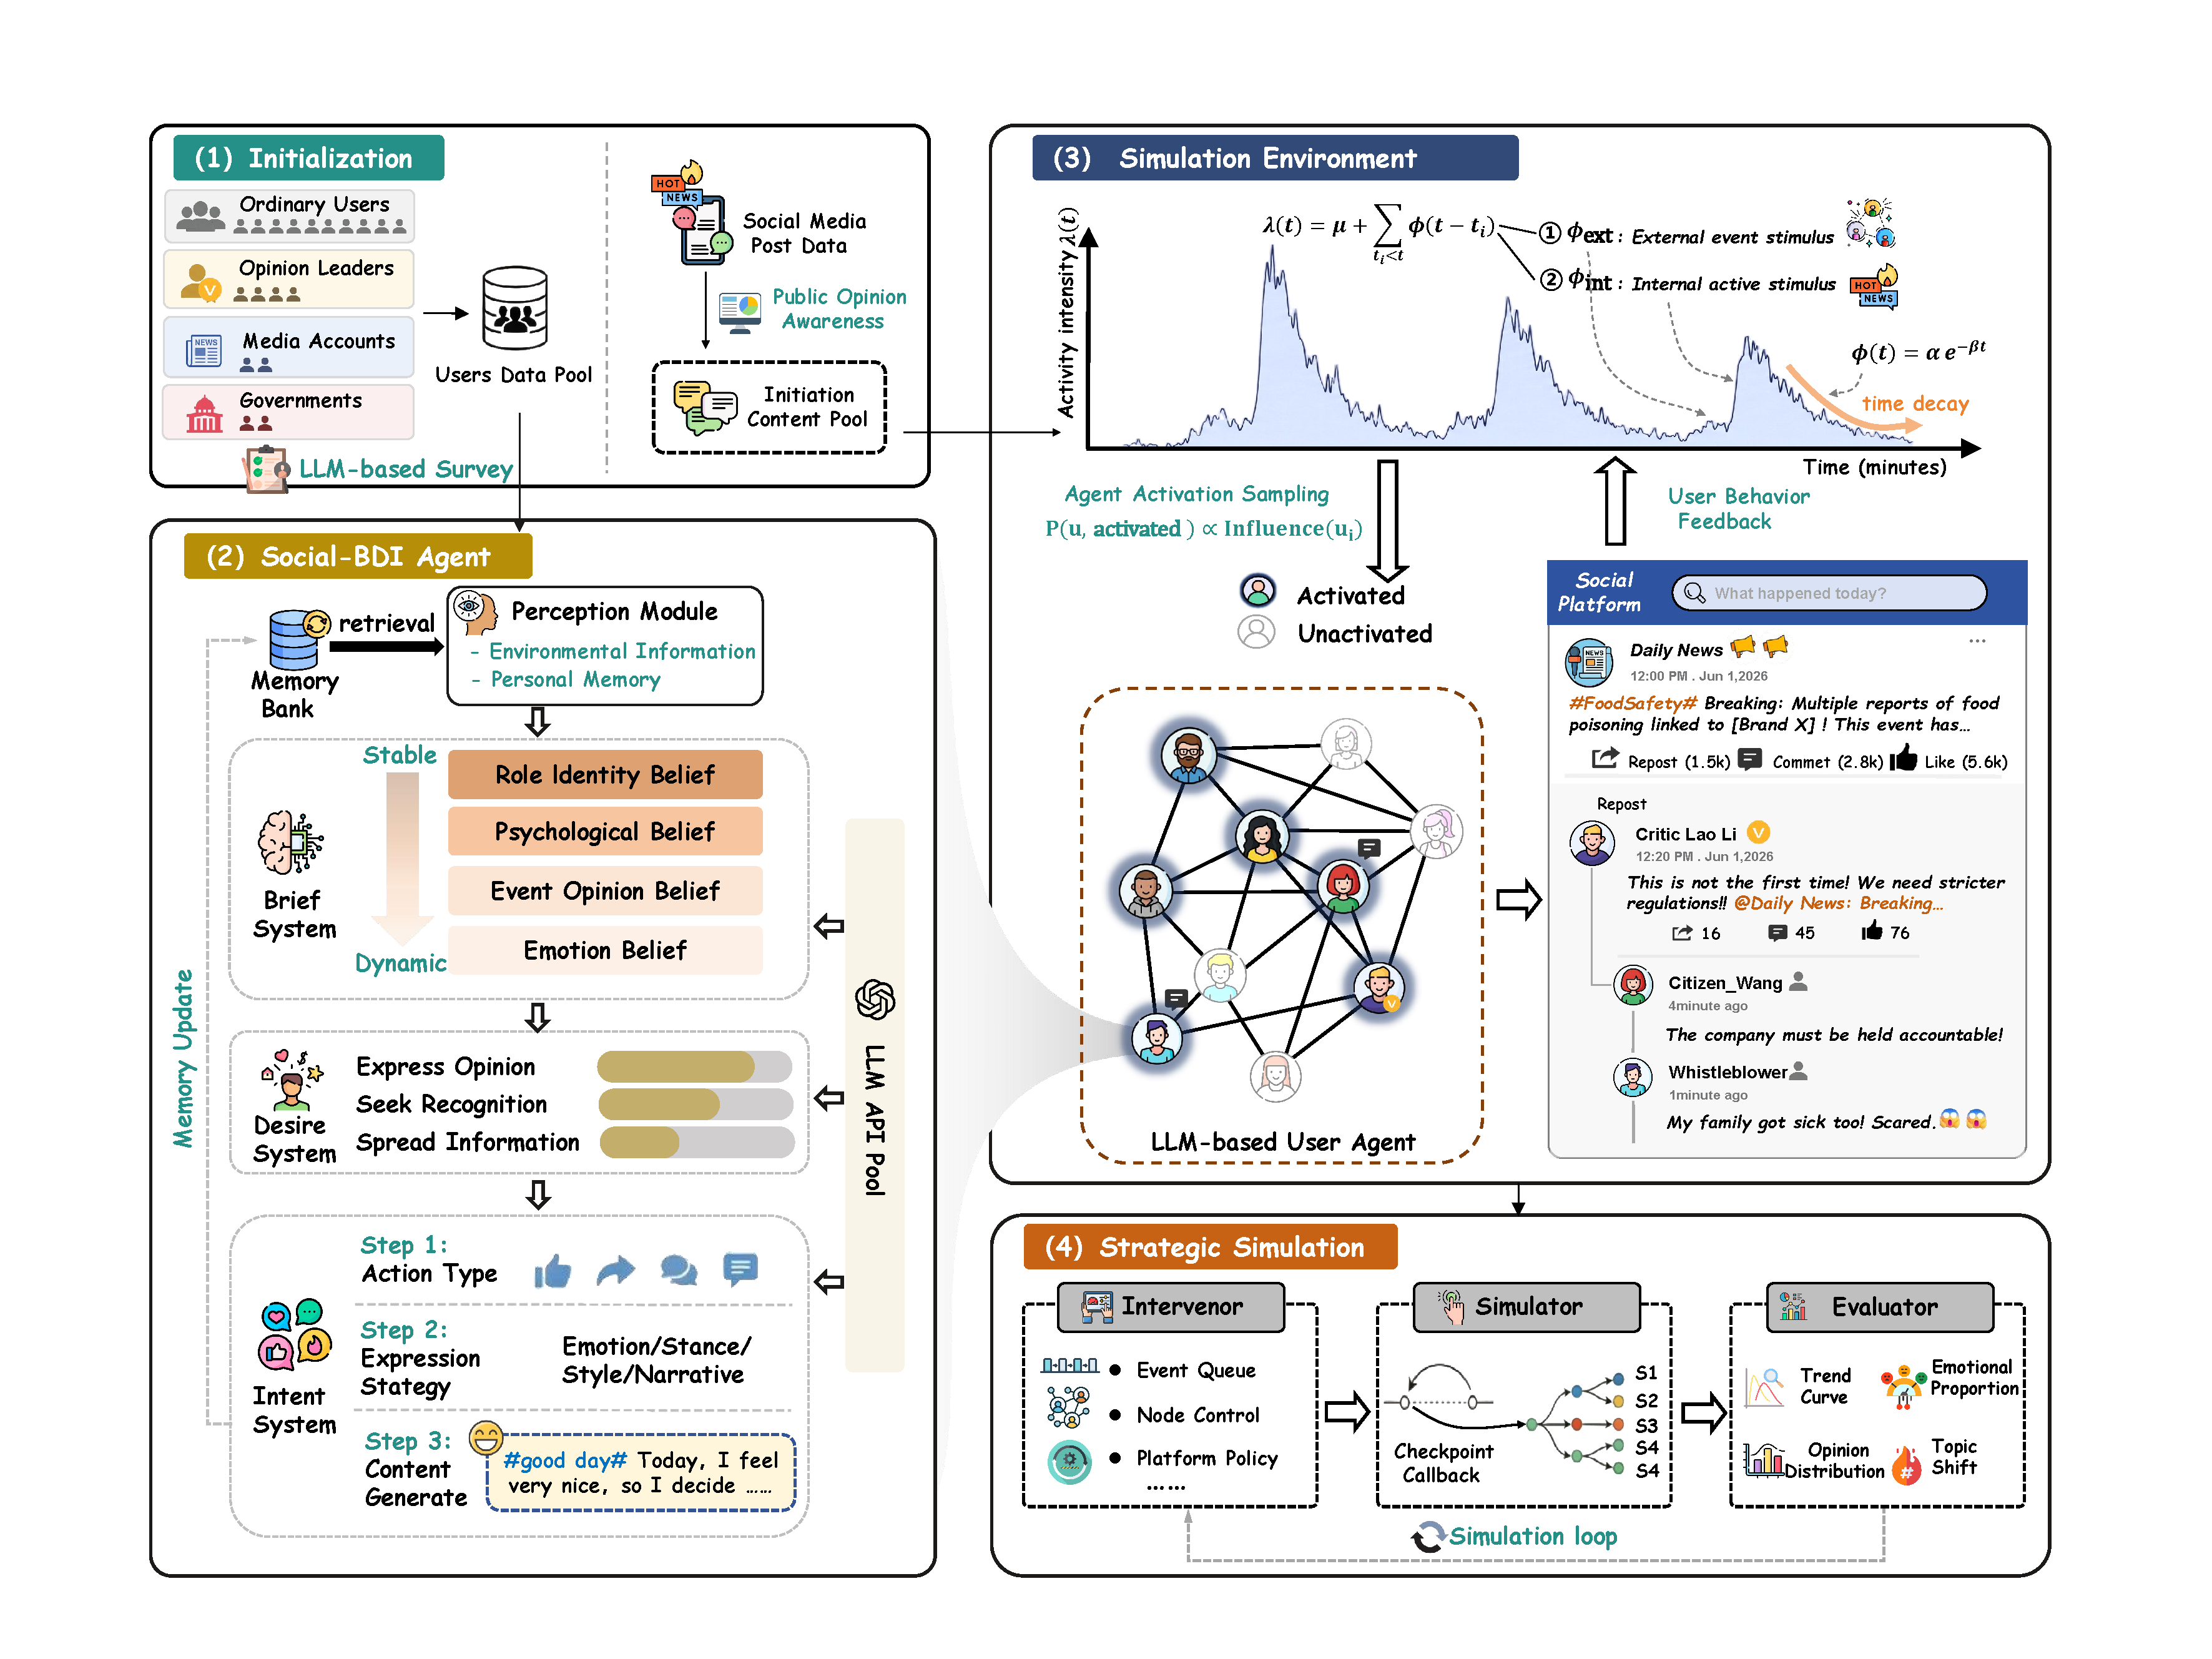
\includegraphics[width=0.85\textwidth]{framework_overview.pdf}
\caption{Overview of the POSIM framework. (1) The initialization module builds agents and the environment from real user profiles and post data. (2) The Social-BDI agent architecture implements the Perception $\to$ Belief $\to$ Desire $\to$ Intention $\to$ Action cognitive decision pipeline. (3) The simulation environment uses a Hawkes self-exciting point process-driven temporal engine to schedule agent activation, while the virtual social media platform provides personalized recommendation and social network interaction. (4) The strategy evaluation module consists of an intervenor, a simulator, and an evaluator.}
\label{fig:framework}
\end{figure*}

\subsection{POSIM Framework Overview}\label{subsec:overview}

The overall architecture of POSIM is illustrated in Figure~\ref{fig:framework}. It consists of three core components: the \textbf{Social-BDI agent architecture}, the \textbf{simulation environment}, and the \textbf{strategy evaluation} module, which respectively address three key questions: ``who participates,'' ``in what environment they participate,'' and ``how simulation supports decision-making.''

At the agent level (Section~\ref{subsec:agent}), POSIM equips each simulated user with a Social-BDI architecture inspired by BDI cognitive theory. This architecture explicitly decomposes the cognitive process into three independent subsystems, belief update, desire generation, and intention planning, each powered by an LLM as its reasoning engine. Together they form a complete and traceable cognitive decision pipeline from environmental perception to behavioral output. The belief subsystem maintains cognitive states across four hierarchical layers: role identity, psychological cognition, event opinions, and emotional arousal, providing personalized cognitive anchoring for downstream decisions. The desire subsystem maps belief states to behavioral motivations with associated intensity weights. The intention subsystem transforms motivations into concrete action types, expression strategies, and textual content through a three-level chain-of-thought mechanism. On this architecture, we further define four heterogeneous agent types, ordinary social users, key opinion leaders (KOLs), media, and government, all sharing the same cognitive pipeline but naturally producing role-specific behaviors through differentiated role-guidance prompts.

At the environment level (Section~\ref{subsec:env}), POSIM constructs a virtual social media environment with social networks and content exposure mechanisms, providing agents with an information setting that closely resembles real platforms. The framework introduces a temporal dynamics engine based on the Hawkes self-exciting point process, which unifies exogenous event shocks and endogenous user interactions into a dynamically evolving collective activity intensity. This enables agents and the environment to remain continuously coupled at minute-level temporal resolution, naturally reproducing the ``outbreak--sustained--decline'' multi-phase evolution pattern of public opinion.

At the strategy evaluation level (Section~\ref{subsec:strategy}), three functional modules, the intervenor, the simulator, and the evaluator, work in concert to support multi-granularity interventions ranging from event injection and node control to platform policy adjustment. A checkpoint-callback mechanism enables counterfactual reasoning, providing quantitative support for governance strategy assessment.

The following sections detail the design and implementation of each core component.


\subsection{Social-BDI Agent Architecture}\label{subsec:agent}

Traditional reactive agents follow a simple perception-to-action pattern, serving as stateless behavior generators that cannot capture the complex cognitive mechanisms underlying social media user decisions. Given that social media behavior is shaped by the interplay of emotional arousal, cognitive biases, and social influence, and that the deep coupling of emotion and intent is a core driver of crisis event evolution~\citep{myint2024crisis_mtl_intent}, we build on the classic BDI (Belief-Desire-Intention) cognitive architecture~\citep{bratman_intention_1987,rao_bdi_1995} and augment it with an affective dimension to propose the Social-BDI agent architecture, which integrates emotional arousal and cognitive biases into a hierarchical cognitive framework. Social-BDI has two defining characteristics. First, each agent maintains explicit self-aware cognitive states, with every decision grounded in observable state changes. Second, the cognitive process itself forms an auditable multi-stage decision chain~\citep{wei_chain_2022} rather than a single black-box call. The cognitive pipeline is formalized as:
\begin{equation}
\underset{\text{Perception}}{P_t} \longrightarrow \underset{\text{Belief}}{B_t} \longrightarrow \underset{\text{Desire}}{D_t} \longrightarrow \underset{\text{Intention}}{I_t} \longrightarrow \underset{\text{Action}}{A_t}
\end{equation}

This architecture uses an LLM as its cognitive reasoning engine and comprises three core modules: the belief subsystem, the desire subsystem, and the intention subsystem. The three subsystems execute sequentially within each decision cycle, with each receiving the output of its upstream counterpart, forming a complete and traceable cognitive pipeline from perception to action.

\subsubsection{Belief Subsystem}

Beliefs constitute an agent's dynamic cognitive representation of the external world and its own internal state, forming the foundation for all downstream reasoning. Social psychology research shows that different cognitive layers exhibit different levels of stability: core personality traits remain highly stable in the short term, whereas opinions on specific events and momentary emotions shift rapidly with incoming information. Based on this cognitive stratification and the characteristics of real social media users, we design a hierarchical belief system $B = \langle B^{id}, B^{psy}, B^{evt}, B^{emo} \rangle$, where the four belief types are ordered by decreasing resistance to cognitive revision.

\textbf{Role identity beliefs} $B^{id}$ encode the agent's inherent baseline cognition, including demographic attributes (gender, region), social attributes (follower count, verification type), and identity attributes (occupation, interest tags). These beliefs remain constant throughout the simulation. During initialization, real user profile information and historical posts are collected from social media platforms, and an LLM performs structured inference to generate role identity descriptions in first-person natural language. This belief layer serves as the personality-consistency anchor and is never updated during simulation.

\textbf{Psychological cognition beliefs} $B^{psy}$ represent the agent's deep psychological traits and cognitive tendencies in the context of public opinion participation. Social psychology research shows that users exhibit typical patterns such as conformity, prejudice, impulsiveness, and obstinacy when engaging with online events~\citep{buckels2014trolls}. Drawing on analysis of user behavior across multiple real opinion events, we categorize psychological traits into representative archetypes such as self-actualization, curiosity-seeking, emotional-venting, anti-establishment, and herd-following. Each archetype is accompanied by predefined psychological cognition entries distilled from large volumes of real opinion data. For instance, the anti-establishment archetype includes cognitions such as ``what mainstream media doesn't report is often the truth'' and ``the wealth of the rich is always suspect,'' while the emotional-venting archetype includes entries such as ``the more dramatic the spectacle, the better'' and ``harsher criticism feels more cathartic.'' These beliefs are stored as structured text lists. During initialization, an LLM samples and adapts entries from the predefined psychological trait pool based on collected real user historical behavior, matching each agent with the psychological cognition combination that best fits its behavioral history. Psychological cognition beliefs remain highly stable during simulation, reflecting the inherent resistance to change of deep psychological traits.

\textbf{Event opinion beliefs} $B^{evt}$ represent the agent's factual understanding, contextual knowledge, and stance toward the entities involved in a specific public opinion event. Unlike the preceding two belief types, event opinion beliefs evolve dynamically as the event unfolds; incoming information, others' opinions, and new developments can all trigger opinion revision or reinforcement. Each event opinion is represented as a structured four-tuple $\langle t, \text{subject}, \text{opinion}, \text{reason} \rangle$. During initialization, an LLM-driven structured deep interview mechanism extracts the user's initial opinion tendencies toward each involved entity based on the user's historical posts prior to the event outbreak.

\textbf{Emotional arousal beliefs} $B^{emo}$ are grounded in the ABC model from cognitive behavioral theory~\citep{ellis_reason_1962}, which emphasizes the mediating role of cognitive appraisal in emotional responses and subsequent behavior. We adopt Ekman's six-dimensional basic emotion framework~\citep{ekman_basic_1992} and represent the emotional state as a continuous vector $\mathbf{e} = [e_{\text{hap}}, e_{\text{sad}}, e_{\text{ang}}, e_{\text{fear}}, e_{\text{sur}}, e_{\text{dis}}]^\top \in [0,1]^6$, corresponding to happiness, sadness, anger, fear, surprise, and disgust. Emotional state updates are driven by three mechanisms. \textbf{Temporal decay} follows the natural dissipation of emotions observed in psychology, where intensity decays exponentially over time:
\begin{equation}
\mathbf{e}_i(t) = \mathbf{e}_i(t_0) \cdot e^{-\lambda_e(t-t_0)}
\end{equation}
\textbf{Content stimulation} refers to the incremental emotional impact of affective tone in recommended content, $\mathbf{e}_i \leftarrow \mathbf{e}_i + \eta \cdot \mathbf{s}_{content}$, where $\eta$ is the stimulation coefficient. \textbf{Social contagion}, grounded in emotional contagion theory for online social networks~\citep{hatfield_emotional_1994,kramer_experimental_2014,fan2023emotional_contagion}, causes an agent's emotions to be influenced by the emotional states of its social neighbors:
\begin{equation}
\mathbf{e}_i \leftarrow (1-\rho) \cdot \mathbf{e}_i + \rho \cdot \bar{\mathbf{e}}_{\text{neighbor}}
\end{equation}
where $\rho$ is the contagion intensity coefficient and $\bar{\mathbf{e}}_{\text{neighbor}}$ is the weighted average of neighbor emotions.

\textbf{Belief update mechanism.} At each time step, the belief subsystem is updated via an LLM call. The update takes dual-channel inputs, external environmental perception $P_t$ and historical behavioral memory $M_t$, and produces updated psychological cognition, event opinion, and emotional arousal beliefs. Historical memory is maintained in a streaming memory store, with retrieval governed by a weighted scoring function that balances temporal recency and semantic relevance:
\begin{equation}
R(m, t) = \alpha_{\mathrm{rec}} e^{-\gamma(t - t_m)} + (1-\alpha_{\mathrm{rec}})\,\text{sim}(q, m),
\label{eq:mmr}
\end{equation}
where $\text{sim}(\cdot,\cdot)$ denotes cosine similarity computed by a pretrained encoder and $\alpha_{\mathrm{rec}}\in[0,1]$ controls the trade-off between recency and relevance. Belief update in real social media users is not a perfectly rational information integration process; it is systematically influenced by multiple cognitive biases. Users tend to selectively accept information consistent with their existing views while ignoring contradictory evidence (\textit{confirmation bias}), to rely disproportionately on initially encountered information when forming opinions (\textit{anchoring effect}), to bypass rational analysis in high-arousal states and make judgments based directly on emotion (\textit{emotion-first reasoning}), and to reduce complex social events to a single cause or individual responsibility (\textit{simplistic attribution}). These cognitive biases are particularly pronounced in public opinion scenarios and serve as key psychological mechanisms driving irrational discourse and group polarization. We therefore explicitly inject these cognitive bias cues into the LLM reasoning process through the prompt, making the agent's belief update process closer to the cognitive profile of real users. The overall belief update is:
\begin{equation}
B_{t+1} = f_{\text{LLM}}(B_t, P_t, M_t, \Phi)
\label{eq:belief_update}
\end{equation}
where $\Phi$ denotes the cognitive bias guidance embedded in the prompt. The update primarily acts on the two rapidly changing layers, $B^{evt}$ and $B^{emo}$, while slowly adjusting $B^{psy}$; $B^{id}$ remains fixed as the identity anchor throughout simulation.

\begin{table}[!t]
\centering
\caption{Hierarchical belief system design. Beliefs are ordered by decreasing cognitive resistance to change: identity beliefs remain fixed, while emotional beliefs update at every step.}
\label{tab:belief}
\scriptsize
\renewcommand{\arraystretch}{1.15}
\begin{tabular}{@{}p{1.15cm}p{1.85cm}p{1.05cm}p{2.3cm}@{}}
\toprule
\textbf{Belief} & \textbf{Representation} & \textbf{Stability} & \textbf{Generation Method} \\
\midrule
$B^{id}$ \newline Identity & First-person natural language narrative & Fixed & LLM init.\ from real user profiles \\
\addlinespace
$B^{psy}$ \newline Psychology & Structured text entry list & Highly stable & LLM + psychological trait pool \\
\addlinespace
$B^{evt}$ \newline Event view & Structured tuple $\langle t, \text{subj}, \text{op}, \text{rsn}\rangle$ & Dynamic & LLM inference at each decision step \\
\addlinespace
$B^{emo}$ \newline Emotion & Six-dim.\ vector $\mathbf{e}\!\in\![0,1]^6$ & Rapid & LLM appraisal + decay \& contagion \\
\bottomrule
\end{tabular}
\end{table}

\subsubsection{Desire Subsystem}

The desire subsystem bridges cognitive states and behavioral motivations, serving as the critical link between ``how the agent understands the world'' and ``what the agent wants to do'' within the Social-BDI architecture. In classical BDI theory, desires are defined as goal states the agent wishes to achieve~\citep{bratman_intention_1987}; in the social media context, we operationalize them as the intrinsic motivations driving user participation in opinion discussions. The participation motivations of social media users are highly diverse and individual-specific: the same piece of news may ignite one user's sense of justice while triggering another's curiosity. This motivational heterogeneity is difficult to cover with fixed rules, so we leverage the commonsense reasoning ability of the LLM to automatically infer behavioral drivers from the agent's current belief state.

At each time step, the desire subsystem receives the updated belief state $B_{t+1}$ and current perception $P_t$ as input, and outputs a set of motivation descriptions with associated intensity weights:
\begin{equation}
D_t = \{(d_1, w_1), (d_2, w_2), \ldots, (d_n, w_n)\}, \quad w_i \in [0, 1]
\end{equation}
where $d_i$ is a natural language description of the motivation type and $w_i$ is the corresponding intensity weight reflecting its drive strength under the current cognitive state. Uses and gratifications theory in communication studies~\citep{katz_uses_1973} posits that audiences are not passive information receivers but actively select and use media content to satisfy their own needs. Inspired by this theory, we recognize that social media users participate in opinion discussions driven by multiple intrinsic needs. Common motivations for ordinary users include emotional venting (releasing frustration and anxiety through expression), justice advocacy (speaking up for disadvantaged parties or pushing for resolution), herd following (joining trending discussions to feel part of the group), and curiosity seeking (tracking new developments to satisfy curiosity). KOLs more commonly exhibit self-expression (showcasing independent views to consolidate influence) and agenda setting (steering public attention to specific issues). The specific combination and intensity distribution of motivations is not preset but dynamically inferred by the LLM based on the belief state. For instance, when the emotional arousal belief $B^{emo}$ shows high anger and the event opinion belief $B^{evt}$ holds a strongly negative stance, emotional venting and justice advocacy motivations tend to receive high weights; when the psychological cognition belief $B^{psy}$ is dominated by curiosity seeking, information acquisition becomes more prominent.

The motivation list provides explicit goal constraints for the downstream intention subsystem. High-weight motivations guide the agent toward matching action types and expression strategies: when emotional venting is the strongest motivation, the agent tends to choose short comments with intense emotional expression; when self-expression dominates, the agent prefers long original posts with a rational-analytical style. The desire generation function is formalized as:
\begin{equation}
D_t = g_{\text{LLM}}(B_{t+1}, P_t)
\end{equation}

The core value of this design lies in the introduction of an explicit motivation layer, so that belief states no longer map directly to behavioral output. Instead, the desire subsystem first generates structured motivation representations, and the intention subsystem then plans concrete actions accordingly. Ablation experiments (Section~\ref{sec:exp}) show that removing the desire module causes the most severe degradation in content-layer metrics, confirming the indispensable role of the motivation layer in driving the faithful reproduction of irrational discourse.

\subsubsection{Intention Subsystem}

The intention subsystem, as the final decision stage of the cognitive pipeline, serves as a hierarchical behavior planner. Following the interaction conventions of social media platforms, we constrain the action categories to atomic operations including liking, direct repost, repost with comment, short comment, long comment, short original post, and long original post. Unlike conventional single-step behavior generation, the intention subsystem adopts a multi-level chain-of-thought mechanism that decomposes behavioral decisions into three progressive reasoning levels.

\textbf{Level 1: Action type and target selection.} Based on the belief state and desire intensity distribution, the LLM selects an action type from the set of atomic operations and determines the target object for interaction. This level decides \textit{what to do} and \textit{to whom}.

\textbf{Level 2: Expression strategy planning.} For actions that require text generation, the system plans an expression strategy along four dimensions: the \textit{emotion dimension} determines the dominant emotion type and intensity level; the \textit{stance dimension} sets the support, opposition, or neutral position toward the target entity and its strength; the \textit{style dimension} selects among rational analysis, sarcasm, emotional attack, empathetic understanding, skeptical inquiry, and other expression styles; the \textit{narrative dimension} chooses among factual enumeration, labeling, call to action, authority citation, and other narrative strategies. Each dimension contains multiple candidate options, and the LLM autonomously selects the most appropriate combination given the current cognitive state. This level decides \textit{how to express}.

\textbf{Level 3: Content generation.} Constrained by the decisions from the preceding two levels, the system generates specific textual content consistent with the agent's role characteristics, including body text, hashtags, and mentions. This level decides \textit{what exactly to say}.

This three-level decomposition provides explicit strategic constraints for content generation, preventing the LLM from defaulting to the averaged, mild text it tends to produce without guidance. Each level's decisions are recorded, making the generation process fully traceable. The overall intention generation is formalized as:
\begin{equation}
I_t = h_{\text{LLM}}(B_{t+1}, D_t, P_t)
\end{equation}
where $I_t = \{(a_j, o_j, s_j, c_j)\}_{j=1}^{m}$ is an action sequence, with each element comprising an action type $a_j$, a target object $o_j$, an expression strategy vector $s_j = (\text{emotion}, \text{stance}, \text{style}, \text{narrative})$, and generated content $c_j$.

\subsubsection{Heterogeneous Agents}

Real public opinion evolution involves complex interactions among ordinary social users, KOLs, media, and government entities~\citep{chen_evolution_2025,wu_public_2023}. All four agent types are built on the same Social-BDI cognitive architecture: they share the identical cognitive pipeline from perception through belief, desire, and intention to action, using the same belief update, desire generation, and intention planning modules. Behavioral differences across agent types arise not from modifications to the cognitive architecture or introduction of additional decision rules, but solely from type-specific role-guidance prompts that inject distinct social role characteristics (such as identity positioning, speaking style, and focus areas), allowing the same architecture to naturally produce differentiated behaviors under different role constraints. This design ensures that behavioral heterogeneity stems from differences in role beliefs rather than architectural differences, preserving the framework's unity and interpretability.

\textbf{Ordinary social users} constitute the overwhelming majority of opinion participants. Their behavior is primarily shaped by the interplay of personal beliefs and immediate emotions, and their language style tends to be colloquial and fragmented, with a propensity for impulsive expression under high emotional arousal.

\textbf{Key opinion leaders (KOLs)}, identified in two-step flow theory~\citep{katz_personal_1955} as critical intermediaries in information flow, possess a large follower base and considerable social influence. Their output tends to exhibit strong independence and agenda-setting effects, exerting significant influence on the belief updates and behavioral decisions of downstream ordinary users.

\textbf{Media agents} serve the social function of information collection and dissemination, emphasizing timeliness, accuracy, and authoritativeness. Their language is relatively formal and restrained; they participate primarily through news reports, event updates, and in-depth commentaries, playing an information-confirming and agenda-framing role at critical event junctures.

\textbf{Government agents} represent the official stance and public governance perspective, fulfilling functions such as policy interpretation, opinion guidance, and information disclosure. They post infrequently but with high authority, typically issuing official statements once an event has reached sufficient scale, producing potentially pivotal effects on opinion trajectories.

The specific behavioral patterns of all four agent types are not hard-coded but autonomously generated by the Social-BDI cognitive pipeline under each type's role-guidance prompt constraints.

Complete cognitive pipeline examples with prompt templates are provided in Appendix~\ref{app:prompts}.

\subsection{Simulation Environment}\label{subsec:env}

The simulation environment is the virtual social media platform in which agents perceive and interact. Its design goal is to faithfully reproduce the information flow mechanisms and temporal dynamics of real social platforms while maintaining computational feasibility. As shown in Figure~\ref{fig:framework}, the environment comprises two major components, the temporal engine and the social network with information flow mechanism, which jointly provide agents with a complete virtual social media experience.

\subsubsection{Temporal Engine}

User activity in real opinion events exhibits highly uneven temporal distributions: an explosive piece of news can trigger thousands of reposts within minutes, while activity drops sharply during lulls. Conventional simulation systems typically adopt a fixed time step with uniform activation, activating a constant number of agents per step. Such a design fails to reproduce the event-driven activity surges characteristic of real opinion dynamics.

To address this, POSIM introduces a \textbf{temporal engine} based on the Hawkes self-exciting point process as the temporal scheduling foundation. The core idea is that collective activity intensity is not a preset constant but a dynamic process jointly driven by exogenous event shocks and endogenous user interactions. Specifically, we adopt the Hawkes self-exciting point process~\citep{hawkes_spectra_1971} to model collective activity intensity. Intuitively, the Hawkes process can be understood through a contagion analogy: each event occurrence briefly elevates the probability of subsequent events, much like a trending post stimulating a burst of participation that gradually subsides. Formally, the conditional intensity function is defined as:
\begin{equation}
\lambda(t) = \mu + \sum_{t_i < t} \phi(t - t_i)
\label{eq:hawkes}
\end{equation}
where $\mu$ is the background activity rate reflecting baseline posting during opinion lulls, and $\phi(t) = \alpha e^{-\beta t}$ is the exponentially decaying excitation kernel capturing the short-term activity boost from each historical event: excitation is strongest immediately after the event and decays exponentially, with contributions from all past events superimposed to form the total intensity at any given moment.

A key design choice is the decomposition of the excitation term into \textbf{exogenous event excitation} $\phi_{ext}$ and \textbf{endogenous activity excitation} $\phi_{int}$ (see Figure~\ref{fig:framework}). Exogenous excitation corresponds to external stimuli such as news releases and official statements, featuring high amplitude and slow decay, capable of substantially elevating collective activity and sustaining a prolonged influence window. Endogenous excitation corresponds to user interactions (reposts, comments, likes), featuring weaker amplitude and faster decay, reflecting the snowball-like self-exciting dynamics of social propagation. Their superposition enables the simulation to naturally produce the ``outbreak--sustained--decline'' activity pattern consistent with real opinion events.

Building on this, we further introduce a circadian rhythm modulation mechanism informed by the temporal patterns of real opinion events. A 24-hour periodic modulation function scales the Hawkes intensity accordingly. Within each simulation step $\Delta t$, the system determines the number of agents to activate via Poisson sampling, $N_t \sim \text{Poisson}(\lambda_{adj}(t)\, N_{\text{scale}})$, and selects specific agents through weighted sampling based on historical activity levels. The full parameter configuration is provided in Appendix~\ref{tab:hawkes_params}.

\subsubsection{Social Network and Information Flow}

After the temporal engine determines which agents to activate at each step, the social network and information flow mechanism jointly determine what each agent sees and which posts attract its attention, directly shaping subsequent interaction behavior.

\textbf{Social network.} The social network provides the underlying infrastructure for information flow. POSIM maintains three directed relationship layers: a follower network, a real-time repost network, and a real-time comment network. The follower network records unidirectional following relationships and defines the scope from which the recommendation system draws relationship-chain content. The repost and comment networks grow dynamically during simulation: whenever an agent executes a repost or comment, the system records the interaction and updates the network topology.

\textbf{Content recommendation.} The recommendation system maintains a global content pool into which all agent-generated posts, comments, and reposts are written in real time, each encoded into a vector representation by a pretrained semantic encoder (BGE-small-zh\footnote{\url{https://huggingface.co/BAAI/bge-small-zh-v1.5}}). To suppress the homogenization tendency of LLM-generated content, the system performs cosine similarity-based semantic deduplication on newly added items. Candidate content is sourced from two channels. The \textbf{relationship channel} retrieves posts from users on the agent's follow list, preserving the information transmission function of social ties. The \textbf{public channel} retrieves from the global content pool, simulating the platform's ability to distribute content across community boundaries. After merging candidates from both channels, the system computes a recommendation score along three weighted dimensions. \textbf{Homophily} $H(u,p)$ measures the cosine similarity between the user's historical interest vector and the candidate's semantic vector, reflecting the filter bubble effect~\citep{cinelli_echo_2021}. \textbf{Popularity} $P(p)$ is based on a normalized weighted score of likes, reposts, and comments, capturing the platform's traffic tilt toward high-engagement content. \textbf{Freshness} $R(p)$ is computed via an exponential time decay function, ensuring recent content receives higher exposure probability. The final recommendation score is:
\begin{equation}
S_{exp}(u, p) = \alpha \cdot H(u, p) + \beta \cdot P(p) + \gamma \cdot R(p)
\label{eq:recommend}
\end{equation}
where $\alpha$, $\beta$, and $\gamma$ are tunable weight parameters (specific values in Appendix Table~\ref{tab:rec_params}). After ranking, the system reserves a fraction of exploration slots for random recommendations to counteract excessive filter bubble effects~\citep{bail_opposing_2018}. A recommendation history mechanism ensures that the same content is not repeatedly pushed to the same user within a short period.

\textbf{Trending topics.} The system automatically tallies the popularity of hashtags that emerge during simulation, periodically updating rankings based on interaction signals and temporal decay. Top-ranked topics are injected into agents' perception inputs, simulating the attention-amplifying effect of trending lists on real platforms.

\subsection{Strategy Evaluation}\label{subsec:strategy}

POSIM is not merely a simulator but a computational experiment platform that supports strategy assessment. In public opinion governance practice, decision-makers frequently need to answer counterfactual questions such as ``if a particular intervention is applied, how will the opinion trajectory change?'' As shown in the lower right of Figure~\ref{fig:framework}, the strategy evaluation framework of POSIM is jointly realized by three functional modules: the \textbf{Intervenor}, the \textbf{Simulator}, and the \textbf{Evaluator}.

\textbf{Intervenor.} The intervenor is a unified interface layer connecting external governance intentions with internal simulation states. It provides three granularities of injection. \textbf{Event queue} broadcasts external events to all agents at specified time points, such as injecting an official statement or breaking news. \textbf{Node control} targets specific agents for precision intervention, for example adjusting a KOL's belief state to simulate a guidance strategy. \textbf{Platform policy} modifies the environment's operating parameters, such as tuning recommendation algorithm weights or restricting the spread of specific content. These three interfaces can be used individually or in combination, providing researchers with comprehensive intervention capabilities from micro-level individuals to macro-level environments.

\textbf{Simulator.} The simulator translates intervention plans into executable computational experiments. Its core mechanism is \textbf{checkpoint callback}: the system periodically saves complete state snapshots during simulation, and researchers can load the historical state from any checkpoint and inject different interventions, thereby generating multiple parallel evolution trajectories from identical initial conditions. This design naturally supports counterfactual reasoning: one simply forks from the same checkpoint, applies different interventions (or no intervention), and directly compares the outcomes.

\textbf{Evaluator.} The evaluator is fully decoupled from the simulation engine. It reads simulation logs through a standardized data interface and performs multi-dimensional quantitative assessment of simulation outputs across metrics including activity curves, sentiment proportions, opinion distributions, and topic migration, providing a comprehensive characterization of opinion evolution states. Evaluation results can be directly fed back to guide the next round of intervention design and optimization.

\textbf{LLM resource scheduling.} Large-scale simulation involves extensive LLM calls, and the framework manages multiple LLM endpoints through a unified API resource pool, supporting mixed multi-model orchestration. For usage routing, the resource pool maintains independent model selection counters for different purposes such as belief update, desire generation, and action decision, supporting assignment of different LLM endpoints per purpose to balance reasoning quality and cost efficiency. To prevent homogenized outputs during large-scale calls, the system applies random perturbation to sampling parameters for each call: temperature perturbation $T' = T + \epsilon_T$ ($\epsilon_T \sim \mathcal{U}(-0.1, 0.1)$), top-$p$ perturbation $p' = p + \epsilon_p$ ($\epsilon_p \sim \mathcal{U}(-0.05, 0.05)$), and random injection of frequency and presence penalties to increase vocabulary and topic diversity. The resource pool also implements endpoint-level concurrency control, round-robin load balancing, automatic fault detection with failover, and call rate limiting.

\textbf{Modular architecture.} A core challenge in opinion simulation research is that different research scenarios demand different cognitive models, temporal dynamics, and evaluation dimensions, and a single monolithic architecture cannot accommodate diverse research objectives. POSIM therefore follows the \textbf{separation of concerns} principle from its inception, encapsulating agent cognition, simulation environment, and strategy evaluation as mutually independent functional modules that communicate solely through semantically clear structured states rather than sharing internal implementation details. This design allows each module to evolve independently. For example, researchers can replace the Social-BDI cognitive architecture with an alternative decision model to explore different cognitive hypotheses while keeping the simulation environment and evaluation system unchanged, or switch the temporal engine to accommodate different time scales while preserving the agent architecture, or plug in new evaluation dimensions to support specific research questions. This research-oriented extensible design enables POSIM to evolve from a single-purpose opinion simulation tool into a general computational experiment platform supporting multiple social simulation paradigms.

% ============================================================
% Section 4: Validation Framework
% ============================================================
\section{Validation Framework}\label{sec:validation}

Our validation framework draws on the classical V\&V (Verification and Validation) principles from systems engineering~\citep{sargent_verification_2013}. We divide model assessment into two complementary dimensions: verification, which asks ``have we built the model correctly?'', and validation, which asks ``are the model's results accurate?'' Based on this principle, validation follows a three-layer progressive process, in which micro-level behavioral mechanism calibration and macro-level emergent phenomenon calibration belong to the verification dimension, while statistical result consistency calibration belongs to the validation dimension.

\textbf{Micro-level behavioral mechanism calibration} (Section~\ref{subsec:micro}) verifies whether agents make cognitively interpretable decisions as designed. This layer focuses on the internal mechanism correctness of the simulation system, examining three progressive dimensions. \textit{Cognitive-behavior chain consistency} checks whether the agent's cognitive pipeline from belief update to behavioral output is complete, coherent, and logically sound, that is, whether each decision can be traced to explicit cognitive evidence. \textit{Personality stability} evaluates whether the agent maintains a behavioral style consistent with its role identity across multiple interaction rounds rather than drifting randomly. \textit{Decision robustness} tests whether the agent's decisions remain stable when inputs are subjected to semantically equivalent perturbations, verifying the effectiveness of the cognitive anchoring mechanism. Micro-level mechanism correctness is the cornerstone of the entire validation system, because only when micro-level mechanisms are correct can macro-level emergence be causally interpretable.

\textbf{Macro-level emergent phenomenon calibration} (Section~\ref{subsec:macro}) verifies whether micro-level mechanisms give rise to macro-level phenomena consistent with social science theories. This layer treats the simulation as a computational experiment and examines whether the system can spontaneously produce group behavioral patterns predicted by social science theories without any explicit macro-level programming. The examination covers four dimensions: multi-phase lifecycle characteristics of public opinion evolution, systematic behavioral heterogeneity across multiple agent types, emotional arousal self-reinforcement and polarization effects, and scale-free network topology with power-law information cascade distributions. The emergence of these phenomena provides indirect yet compelling evidence for the soundness of the micro-level mechanisms.

\textbf{Statistical result consistency calibration} (Section~\ref{subsec:stat}), following mechanism calibration, verifies whether simulation outputs statistically reproduce real opinion dynamics. This layer systematically compares simulation outputs against real opinion data across three dimensions and nine quantitative metrics: the behavior layer (action type distribution and activity curves), the content layer (discourse irrationality distribution, lexical diversity, and sentiment orientation), and the topology layer (network structure and information cascade patterns), thereby establishing the statistical credibility of the simulation.

% ============================================================
% Section 5: Experiments
% ============================================================
\section{Experiments}\label{sec:exp}

\subsection{Datasets}

We collect three real-world public opinion event datasets from the Sina Weibo platform, covering the full interaction chain of original posts, reposts, and comments. The three events belong to the categories of social controversy, campus incident, and food safety, respectively, spanning diverse opinion patterns from short-term eruptions to long-cycle multi-phase evolution. The \textbf{Luxury Earring event} (LE) occurred in May 2025, when green earrings worn by an actress in her coming-of-age ceremony photos were identified by netizens as a luxury brand item worth approximately 2.3 million yuan. This triggered intense public debate over celebrity ostentation and youth value orientation, with the topic trending on Weibo multiple times in a typical short-term eruption pattern. The \textbf{WHU Library event} (WL) originated from a sexual harassment accusation dispute at Wuhan University's library study area in July 2023; in July 2025, the first-instance court ruling reignited public discourse, with large-scale discussion centering on judicial fairness, campus safety, and gender issues, exhibiting a long-cycle multi-phase evolution from dormancy to resurgence. The \textbf{Xibei Prepared Food event} (XF) was triggered in September 2025 when a prominent internet entrepreneur publicly accused the Xibei restaurant chain of extensive use of prepared food. The ongoing confrontation between both parties fueled widespread public concern over food safety and consumer rights, exhibiting a sustained fermentation pattern driven by multi-party contestation.

We select the core period of peak outbreak and evolution for each event for precise simulation, maximizing the information density of simulation within limited computational resources. Descriptive statistics after deduplication, low-activity user filtering, and irrelevant content cleaning are presented in Table~\ref{tab:dataset}. The simulation temporal resolution is 10 minutes per step. Agent belief initialization is based on each user's historical posting content before the simulation start time, sequentially constructing role identity beliefs, psychological cognition beliefs, event opinion beliefs, and the initial emotion vector to form a complete personalized Social-BDI belief system.

\begin{table}[!t]
\centering
\caption{Descriptive statistics of three public opinion event datasets.}
\label{tab:dataset}
\footnotesize
\renewcommand{\arraystretch}{1.05}
\begin{tabular}{@{}lccccc@{}}
\toprule
\textbf{Event} & \textbf{\#Users} & \textbf{\#Posts} & \textbf{Duration} & \textbf{\#Steps} & \textbf{Category} \\
\midrule
LE & 1,530 & 34,218 & ${\sim}$46h & 276 & Social Controversy \\
WL & 1,843 & 51,647 & ${\sim}$190h & 1,140 & Campus Incident \\
XF & 1,987 & 14,892 & ${\sim}$71h & 426 & Food Safety \\
\bottomrule
\end{tabular}
\par\vspace{2pt}
{\scriptsize\fontspec{Times New Roman}\selectfont
\textit{Note}: LE = Luxury Earring; WL = WHU Library; XF = Xibei Prepared Food.}
\end{table}

\subsection{Micro-Level Behavioral Mechanism Validation}\label{subsec:micro}


\subsubsection{Comparison Methods}

Micro-level validation focuses on the cognitive decision quality of individual agents, so all comparison methods are evaluated under identical input conditions to examine the effect of different cognitive architectures on decision interpretability, personality consistency, and robustness. Four decision methods are tested. \textbf{Direct-Nothink} uses a non-reasoning model, Qwen2.5-7B-Instruct\footnote{\url{https://huggingface.co/Qwen/Qwen2.5-7B-Instruct}}, concatenating environmental information and role descriptions into a single prompt that directly requests behavioral decisions without any explicit cognitive reasoning. \textbf{Direct-Think} upgrades the model to the stronger reasoning-capable Qwen3-8B\footnote{\url{https://huggingface.co/Qwen/Qwen3-8B}}, with the same single-prompt direct output approach. \textbf{CoT} uses the same base model as Social-BDI (Qwen2.5-7B-Instruct) and performs belief inference, desire analysis, and behavioral decision in a single LLM call through chain-of-thought prompting, completing all three stages sequentially within the same context window rather than as independent modular calls. \textbf{Social-BDI} is the proposed method, also using Qwen2.5-7B-Instruct as its base model. It decomposes the cognitive process into three independent modules for belief update, desire generation, and intention planning, with each module executed as a separate LLM call and information passed between modules through structured intermediate states.

\subsubsection{Evaluation Setup and Results}

We randomly sample $N=100$ users as agents and run the simulation for $T=12$ rounds, with all four methods operating under identical conditions. Three evaluation dimensions are assessed. \textbf{Cognitive-behavior chain consistency} is scored on a 0--5 scale across four sub-dimensions: cognitive chain completeness, emotional dynamics rationality, motivation-behavior alignment, and information integration capability. \textbf{Personality stability} evaluates the similarity (0--1) between an LLM-inferred personality description reconstructed from the agent's behavioral trajectory and the original personality profile. \textbf{Decision robustness} assesses decision stability (0--1) after semantically equivalent perturbations to the input. All three evaluations are produced by LLM prompts under stable hyperparameters. The results are reported in Table~\ref{tab:micro}.

\begin{table}[!t]
\centering
\caption{Micro-level behavioral mechanism validation results (mean$\pm$std).}
\label{tab:micro}
\renewcommand{\arraystretch}{1.05}
\resizebox{\columnwidth}{!}{%
\scriptsize
\begin{tabular}{@{}lccc@{}}
\toprule
\textbf{Method} & \makecell{\textbf{Cognitive-Behavior}\\\textbf{Chain Consistency} (0--5)\,$\uparrow$} & \makecell{\textbf{Personality}\\\textbf{Stability} (0--1)\,$\uparrow$} & \makecell{\textbf{Decision}\\\textbf{Robustness} (0--1)\,$\uparrow$} \\
\midrule
Direct-Nothink & 1.47$\pm$0.50 & 0.478$\pm$0.263 & 0.629$\pm$0.240 \\
Direct-Think & 1.75$\pm$0.43 & 0.448$\pm$0.269 & 0.603$\pm$0.299 \\
CoT & 3.09$\pm$0.29 & 0.516$\pm$0.272 & 0.541$\pm$0.356 \\
\rowcolor{grayrow}
\textbf{Social-BDI (Ours)} & \textbf{4.64}$\pm$\textbf{0.48} & \textbf{0.661}$\pm$\textbf{0.215} & \textbf{0.695}$\pm$\textbf{0.213} \\
\bottomrule
\end{tabular}%
}
\end{table}

Social-BDI outperforms all baselines across all three dimensions. The cognitive-behavior chain consistency score of 4.64 significantly exceeds CoT's 3.09 ($p < 0.001$), indicating that the hierarchical cognitive architecture produces more complete, coherent, and logically sound decision chains. Personality stability and decision robustness are likewise highest, confirming the effectiveness of the belief anchoring mechanism. Direct-Think, despite using a stronger reasoning-capable model, performs even worse than Direct-Nothink on personality stability and decision robustness due to the lack of structural cognitive constraints, demonstrating that raw model reasoning capability alone cannot substitute for explicit cognitive architecture design. Although CoT incorporates cognitive reasoning within a single call, its decision robustness is the lowest (0.541) among all methods, indicating that single-call reasoning lacks stable state anchoring, whereas Social-BDI provides cognitive anchoring through explicit, modularized belief states.

\subsection{Macro-Level Emergent Phenomena}\label{subsec:macro}

\subsubsection{Public Opinion Lifecycle}

\begin{figure}[!t]
\centering
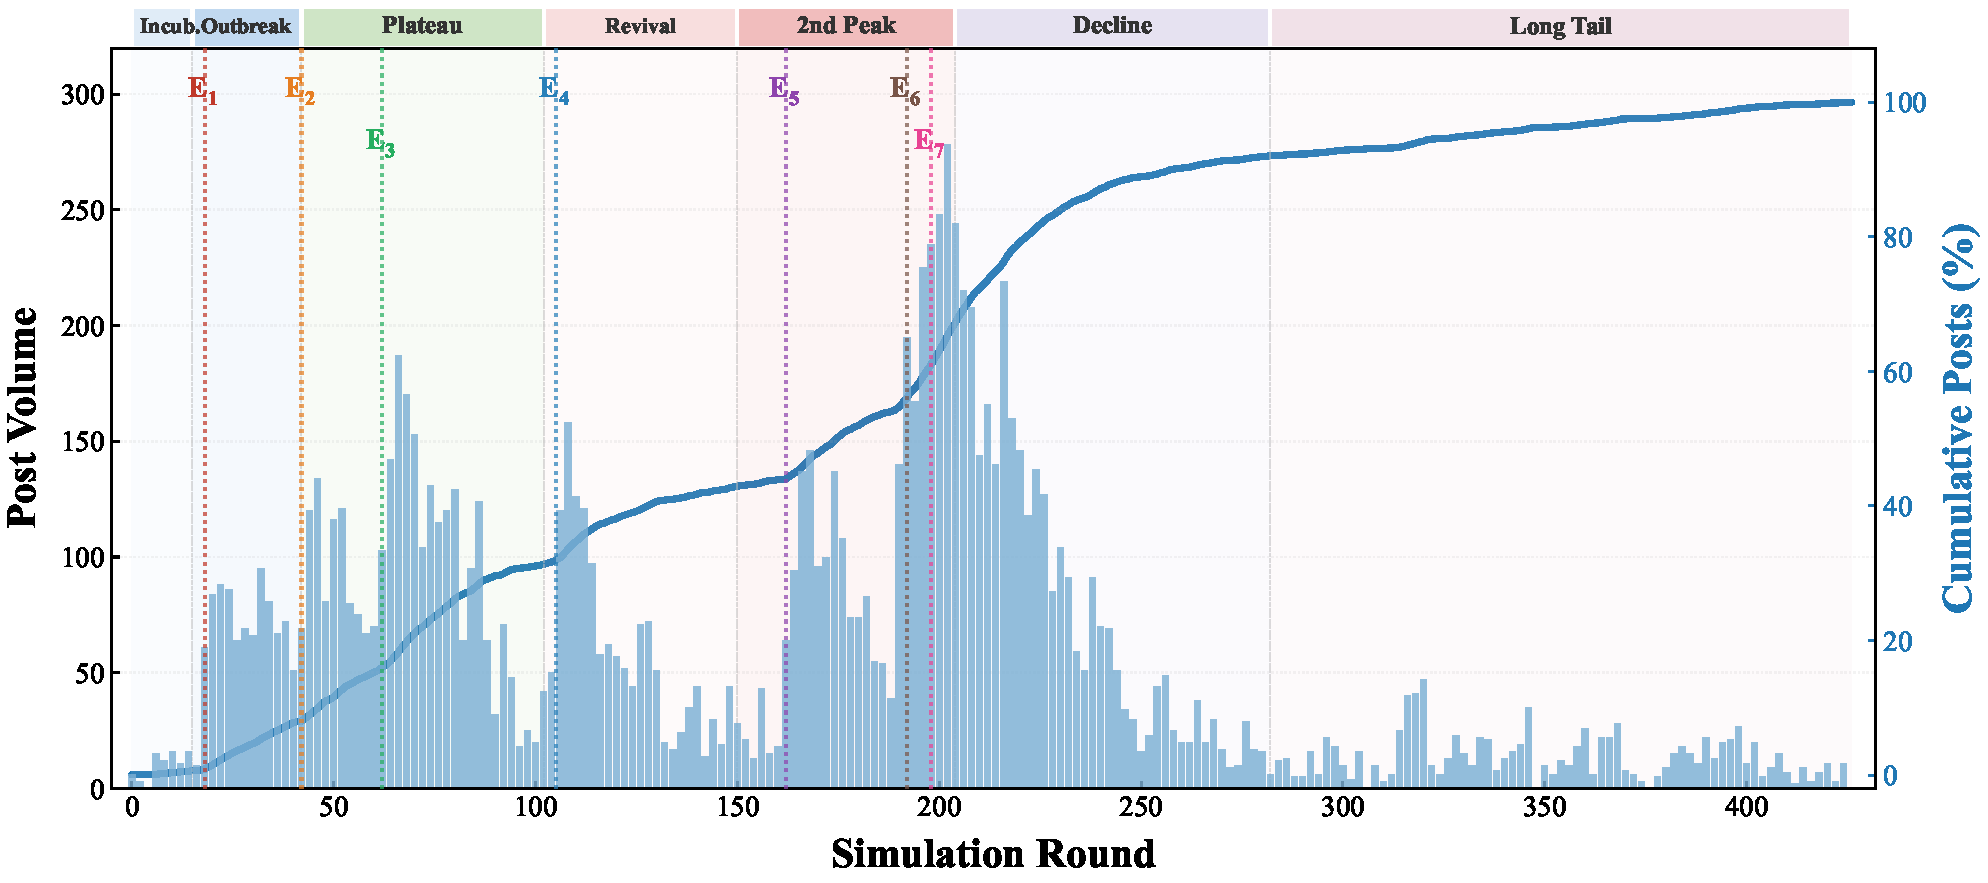
\includegraphics[width=\columnwidth]{fig_lifecycle_paper.pdf}
\caption{Simulated public opinion lifecycle, showing posting volume (bar chart, left axis) and cumulative posting percentage as an S-curve (solid line, right axis). $E_1$--$E_7$ mark exogenous event injection points.}
\label{fig:lifecycle}
\end{figure}

Public opinion lifecycle theory holds that the evolution of online opinion events is neither uniform nor monotonic but exhibits stage-specific patterns~\citep{guo_stochastic_2024,chen_evolution_2025}. A typical lifecycle includes an outbreak phase (event exposure triggers concentrated public attention with rapidly rising activity), a plateau phase (activity stabilizes or fluctuates mildly), a possible resurgence phase (new stimuli trigger secondary outbreaks), and a decline phase (public attention shifts and activity gradually recedes). Not all opinion events follow the same stage sequence: short-burst events may transition directly from outbreak to decline, while multi-party contestation events may undergo multiple resurgence cycles. This section uses the simulation results of the Xibei Prepared Food event (XF) to verify whether POSIM can spontaneously produce a lifecycle pattern consistent with the event's actual development.

As shown in Figure~\ref{fig:lifecycle}, the simulation clearly exhibits a multi-phase lifecycle from outbreak through plateau, resurgence, to decline, with each phase transition traceable to a specific exogenous event as its causal driver. After $E_1$ (exposure of a leaked kitchen video triggering a food safety crisis), posting volume rises sharply, entering the outbreak phase. After $E_2$ (the internet entrepreneur announces a temporary ceasefire), activity drops noticeably, entering the plateau phase. $E_3$ (the restaurant industry debates the definition of prepared food) sustains moderate discussion but does not trigger a large-scale outbreak. $E_4$ (leaked group chat screenshots in which the founder calls the entrepreneur a ``cyber thug'') reignites discussion, breaking the ceasefire deadlock. $E_5$ (state media collectively weigh in) triggers the highest activity peak across the entire simulation, exhibiting a classic resurgence effect and the amplification typically seen when official media set the tone. The cumulative posting percentage follows an S-shaped growth curve, closely matching the S-curve diffusion theory in communication studies~\citep{kong_exploring_2020}.

It is worth emphasizing that this multi-phase lifecycle pattern is not driven by preset rules but emerges spontaneously from the synergy of two mechanism layers. At the \textbf{environment layer}, the self-exciting mechanism of the Hawkes process causes collective activity to exhibit an ``excitation--amplification--decay'' dynamic response after exogenous event injection: exogenous events raise the baseline activation intensity, and event-related content published by agents further amplifies collective activity through the self-exciting term $\sum \alpha e^{-\beta(t-t_i)}$, forming a positive feedback loop; as event stimulation fades and self-excitation decays, activity naturally recedes. At the \textbf{agent layer}, the Social-BDI cognitive architecture causes agents to produce differentiated cognitive responses to different event types. For instance, a food safety crisis ($E_1$) and personal attack screenshots ($E_4$) elicit strong emotional arousal and belief conflict, driving high-density participation; in contrast, a technical industry debate ($E_3$) has weaker cognitive impact on ordinary users, sustaining only moderate discussion. This synergy between environment-driven and cognition-driven dynamics enables the simulation to naturally reproduce the nonlinear mapping between event types and public response intensity observed in real opinion dynamics.

\subsubsection{Multi-Agent Behavioral Heterogeneity}

\FloatBarrier
\begin{figure}[!t]
\centering
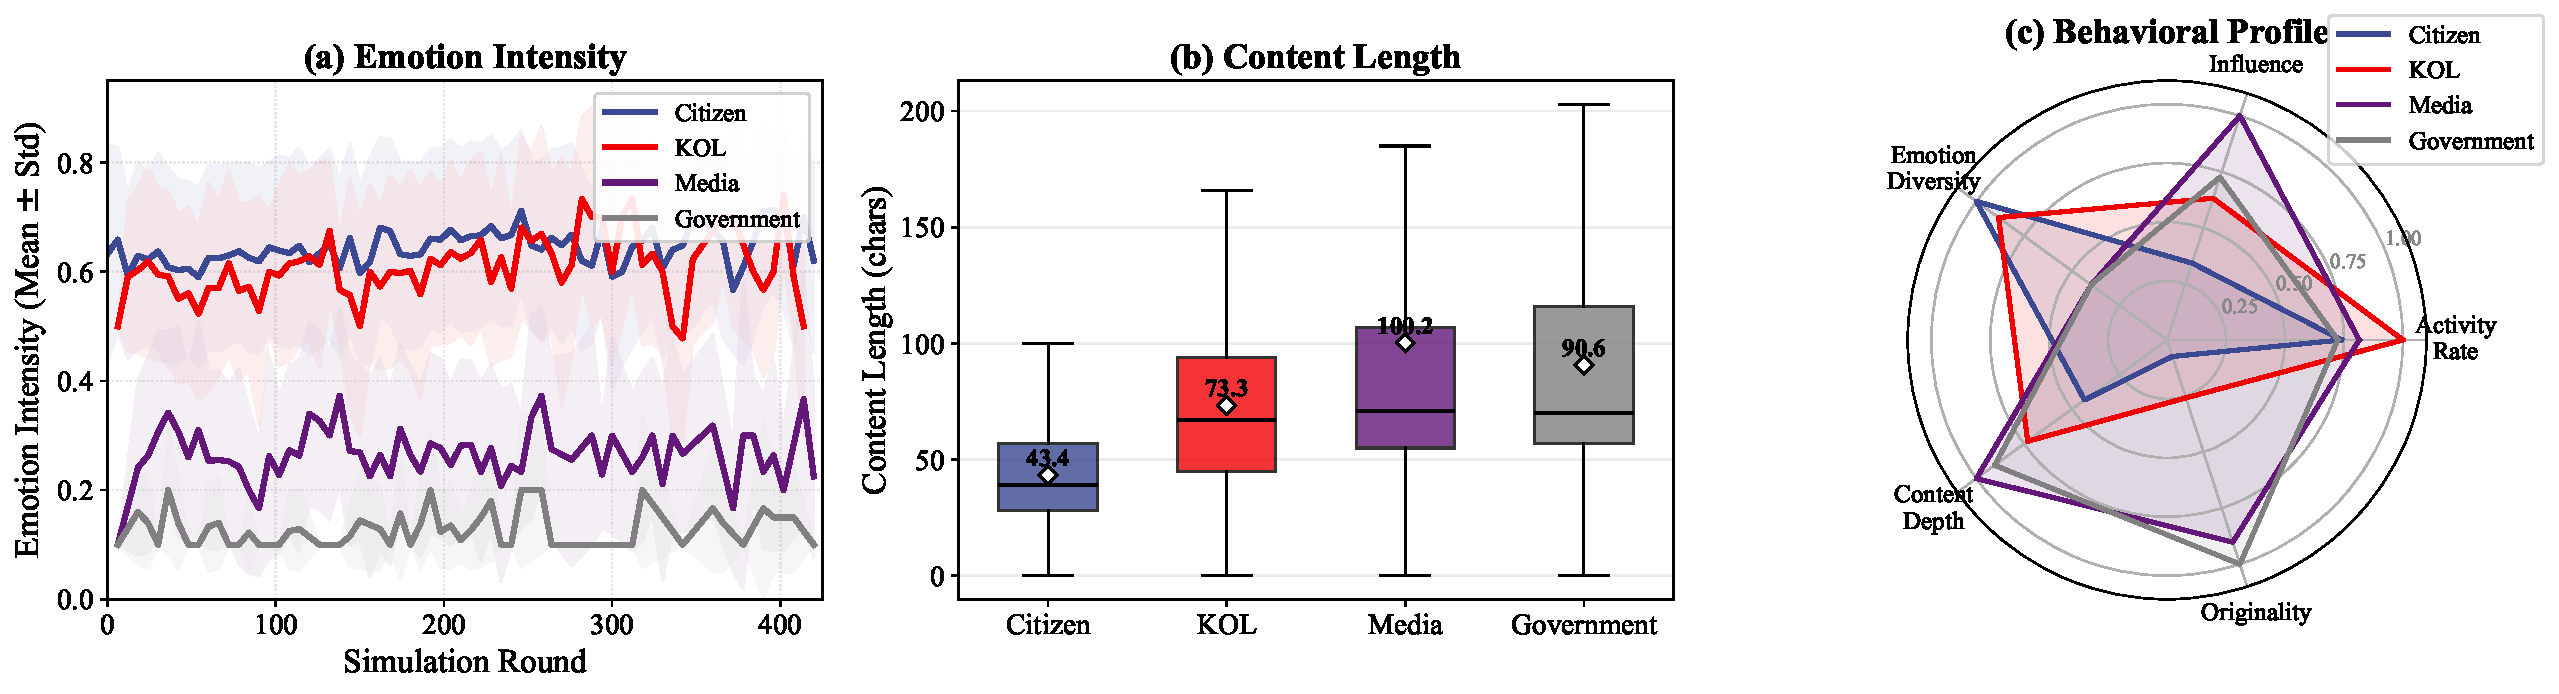
\includegraphics[width=\columnwidth]{fig_paper_heterogeneity.pdf}
\caption{Behavioral heterogeneity across four agent types. (a) Temporal evolution of emotional intensity. (b) Content length distribution. (c) Multi-dimensional behavioral profile radar chart.}
\label{fig:heterogeneity}
\end{figure}

Figure~\ref{fig:heterogeneity} illustrates the systematic heterogeneity that emerges across four agent types from three perspectives: emotional intensity, content length, and multi-dimensional behavioral profile. In the emotional intensity dimension, Citizen and KOL agents maintain average emotional intensities of 0.645 and 0.603 respectively, consistently in the high-arousal range with sharper fluctuations following event stimuli. Media and Government agents remain stable in the low-arousal range, exhibiting a stratified pattern of public emotionality versus official neutrality consistent with the widely observed real-world phenomenon of ``public outrage, official restraint.'' In the content length dimension, Media and Government agents produce significantly longer content on average than Citizens, reflecting the more detailed and structured output of official and media agents. On the radar chart, the four agent types form distinctly shaped polygons: Citizens are prominent in the emotional and interaction frequency dimensions, KOLs lead in influence and content output volume, Media excel in content quality and neutral expression, and Government agents are characterized by low-frequency but high-authority postings. These heterogeneity patterns are not manually coded but emerge naturally from the differentiated role beliefs and motivation weights within the Social-BDI architecture, validating the framework's effectiveness in multi-agent heterogeneity modeling.

\subsubsection{Emotional Arousal and Polarization Effects}

Drawing on emotional arousal theory~\citep{berger_what_2012} and the emotional contagion hypothesis~\citep{hatfield_emotional_1994}, we validate the simulation from two dimensions: arousal self-reinforcement and emotional contagion (Table~\ref{tab:emotion}). The arousal self-reinforcement dimension includes three metrics: (1) \textit{high-arousal trend coefficient} $\beta$, obtained by linear regression on the proportion of high-arousal emotions (strongly stimulating emotions such as anger and excitement) over time, where $\beta>0$ indicates an upward trend; (2) \textit{high-arousal emotion ratio}, the proportion of high-arousal emotions across the entire simulation, verifying whether they dominate the opinion discourse; (3) \textit{high/low arousal intensity ratio}, comparing average intensities between high- and low-arousal emotions. The emotional contagion dimension includes two metrics: (4) \textit{comment-chain emotion consistency}, the proportion of adjacent comments within each comment chain that share the same emotional polarity, where high consistency indicates upstream-to-downstream contagion; (5) \textit{escalation/de-escalation ratio}, the ratio of emotion transitions from low to high arousal versus high to low arousal, where a value greater than 1 indicates a ratchet-like accumulation pattern where emotions tend to intensify rather than subside during interactions.

\begin{table}[!t]
\centering
\caption{Emotional arousal theory validation metrics.}
\label{tab:emotion}
\renewcommand{\arraystretch}{1.0}
\resizebox{\columnwidth}{!}{%
\scriptsize
\begin{tabular}{@{}p{1.5cm}p{3.0cm}cc@{}}
\toprule
\textbf{Dimension} & \textbf{Metric} & \textbf{Sim.\ Result} & \textbf{Theoretical Expectation} \\
\midrule
\multirow{3}{1.5cm}{Arousal Self-Reinforcement$^{\rm a}$}
 & High-arousal trend coeff.\ $\beta$ & $3.41{\times}10^{-4}$\,($p{<}.001$) & $\beta > 0$ \\
 & High-arousal emotion ratio & 73.5\% & Dominant \\
 & High/low arousal intensity ratio & 2.0$\times$ & $>1$ \\
\midrule
\multirow{2}{1.5cm}{Emotional Contagion$^{\rm b}$}
 & Comment-chain emotion consistency & 0.772 & $\gg$ random baseline \\
 & Escalation/de-escalation ratio & 4.78 & $>1$ (ratchet effect) \\
\bottomrule
\end{tabular}%
}
\vspace{3pt}
{\footnotesize $^{\rm a}$~\citet{berger_what_2012};\quad $^{\rm b}$~\citet{hatfield_emotional_1994}}
\end{table}

The simulation results show that high-arousal emotions exhibit a significant upward trend over the course of the simulation, ultimately reaching 73.5\%, consistent with existing findings that high-arousal emotions more readily promote content sharing and propagation~\citep{berger_what_2012}. Comment-chain emotion consistency reaches 0.772. Comparing the frequency of emotion transitions from low to high arousal against the reverse direction yields a ratio of 4.78, indicating that emotions tend to intensify rather than subside during interactions, exhibiting a clear ratchet-like accumulation pattern that provides support for the emotional contagion hypothesis~\citep{hatfield_emotional_1994}.
We further define a polarization index $\text{PI} = 1 - H/H_{\max}$. As shown in Figure~\ref{fig:polarization}, the polarization index rises from 0.41 in the early phase to 0.67 in the late phase (a 63\% increase, $p < 0.001$), indicating that the emotion distribution in the system progressively concentrates toward a few dominant emotions as the simulation advances, a trend consistent with the theoretical expectation of emotional convergence and reinforcement under echo chamber conditions~\citep{cinelli_echo_2021}.

\begin{figure}[!t]
\centering
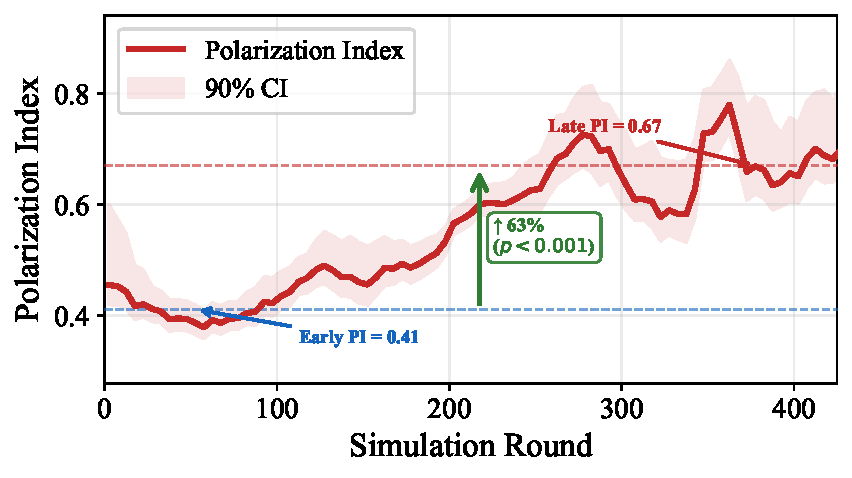
\includegraphics[width=0.85\columnwidth]{fig_paper_polarization.pdf}
\caption{Evolution of the emotional polarization index (PI) over simulation rounds. The solid line denotes the PI mean, the shaded region represents the 90\% bootstrap confidence interval, and dashed lines mark early-stage and late-stage means.}
\label{fig:polarization}
\end{figure}

\subsubsection{Scale-Free Topology and Cascade Power Law}

\begin{figure}[!t]
\centering
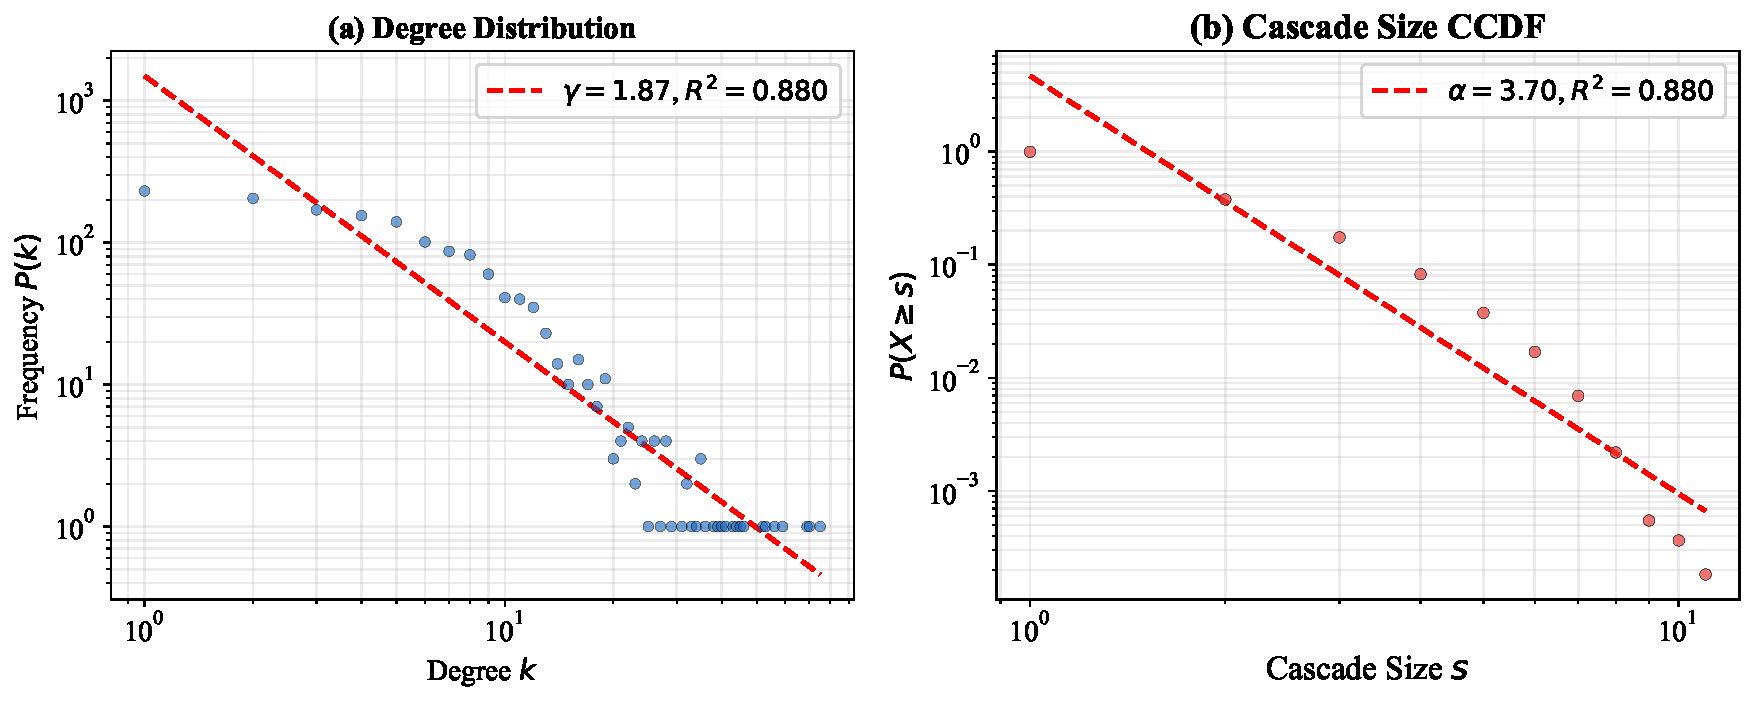
\includegraphics[width=\columnwidth]{fig_paper_powerlaw.pdf}
\caption{Topological properties of the interaction network. (a) Power-law fit of the degree distribution $P(k) \sim k^{-\gamma}$. (b) CCDF of cascade size $P(X \geq s) \sim s^{-\alpha}$.}
\label{fig:powerlaw}
\end{figure}

Degree distributions and information cascade sizes in real social networks generally follow power-law distributions~\citep{barabasi_albert_1999}. As shown in Figure~\ref{fig:powerlaw}(a), the power-law exponent of the interaction network's degree distribution is $\gamma = 1.87$ ($R^2 = 0.880$), falling within the commonly reported range of $1.5 < \gamma < 3$ for real social networks, indicating that the simulated network exhibits typical scale-free characteristics where a few KOL nodes form high-degree hubs while the majority of ordinary users have only sparse connections. As shown in Figure~\ref{fig:powerlaw}(b), the complementary cumulative distribution function (CCDF) of information cascade sizes yields $\alpha = 3.70$ ($R^2 = 0.880$), indicating that the vast majority of repost cascades are small in scale, but occasional explosive propagation events involve large numbers of users, consistent with the long-tail phenomenon on real Weibo where ``most posts go unnoticed while a few go viral.''

\subsection{Statistical Result Calibration}\label{subsec:stat}

This section directly compares simulation outputs against three real opinion events across three dimensions: the \textbf{behavior layer} (action type distribution and activity curves), the \textbf{content layer} (discourse irrationality, lexical diversity, and sentiment orientation), and the \textbf{topology layer} (network structure and information cascades).

\subsubsection{Comparison Methods}

Statistical calibration examines whether the group behavior emerging from large-scale multi-agent interaction is statistically consistent with real data. The comparison methods therefore require end-to-end multi-step simulation in the complete simulation environment. Three baselines are tested. \textbf{Rule-based ABM} uses traditional rule-driven simulation in which each agent samples its action type from a predefined behavioral probability distribution according to its role type (ordinary user, KOL, media, government), with the entire decision process based on preset rules without any LLM involvement. \textbf{POSIM w/ LLM} removes the Social-BDI cognitive architecture within the POSIM simulation environment; after receiving recommended content, the agent generates behavioral decisions and content in a single LLM step without explicit belief update or desire reasoning. \textbf{POSIM w/ CoT} replaces the three independent modules of Social-BDI with a single chain-of-thought reasoning call, completing the entire cognitive-to-behavioral process within a single LLM invocation while retaining all other aspects of POSIM.

\subsubsection{Evaluation Metrics}

Evaluation quantitatively compares simulation outputs against real data across behavior, content, and topology layers, comprising nine metrics in total.

The \textbf{behavior layer} measures the consistency of agent group behavioral patterns with real users across three metrics. BType JSD uses Jensen-Shannon divergence to measure the difference between simulated and real behavioral type probability distributions, defined as $\text{JSD}(P \| Q) = \tfrac{1}{2} D_{\text{KL}}(P \| M) + \tfrac{1}{2} D_{\text{KL}}(Q \| M)$, where $M = (P + Q)/2$. Act.\,$\rho$ measures the Pearson correlation between simulated and real activity time series. Act.\,RMSE measures the point-wise root mean squared error between the two activity curves.

The \textbf{content layer} measures the semantic match between generated text and real content across three metrics. Irrat.\,Sim.\ classifies discourse into irrational, rational, and neutral categories based on keywords and computes the similarity between simulated and real distributions; this metric directly reflects whether the simulation can reproduce the irrational discourse landscape driven by emotions and cognitive biases in real opinion events, which is a core manifestation of the belief module's behavioral activation in the Social-BDI architecture. $|\Delta\text{TTR}|$ measures the difference in lexical richness between simulated and real text, where TTR is the Type-Token Ratio. $|\Delta\bar{S}|$ measures the overall deviation between simulated and real group sentiment means, where $S$ is the sentiment score output by the SnowNLP sentiment analysis library (positive values indicate positive sentiment, negative values indicate negative sentiment).

The \textbf{topology layer} measures the emergent network structure and propagation patterns from simulation across three metrics. Net.\,Sim.\ compares topological features between simulated and real interaction networks. Casc.\,Sim.\ compares the statistical distributions of information cascade sizes. Casc.\,PL compares the proximity of power-law fitting parameters for cascade sizes.

Within each layer, average scores are obtained by normalizing smaller-is-better metrics via $1{-}x$ and then averaging with larger-is-better metrics.

\subsubsection{Calibration Results}

\begin{table*}[!t]
\centering
\caption{Statistical calibration results across three events (LE\,=\,Luxury Earring, WL\,=\,WHU Library, XF\,=\,Xibei Prepared Food). \textbf{Bold}: best per dataset; \na: not applicable. \textcolor{gaingreen}{Green}: gain of POSIM over the second-best method.}
\label{tab:calibration}
\vspace{2pt}
\renewcommand{\arraystretch}{1.05}
\resizebox{\textwidth}{!}{%
\footnotesize
\begin{tabular}{@{}cl cccc cccc cccc@{}}
\toprule
\multirow{2}{*}{\textbf{Data}} & \multirow{2}{*}{\textbf{Method}}
& \multicolumn{4}{c}{\textbf{Behavior Layer}}
& \multicolumn{4}{c}{\textbf{Content Layer}}
& \multicolumn{4}{c}{\textbf{Topology Layer}} \\
\cmidrule(lr){3-6} \cmidrule(lr){7-10} \cmidrule(lr){11-14}
& & \makecell{BType\\JSD\,$\downarrow$} & \makecell{Act.\\$\rho$\,$\uparrow$} & \makecell{Act.\\RMSE\,$\downarrow$} & \makecell{Avg.\\$\uparrow$}
& \makecell{Irrat.\\Sim.\,$\uparrow$} & \makecell{$|\Delta\text{TTR}|$\\$\downarrow$} & \makecell{$|\Delta\bar{S}|$\\$\downarrow$} & \makecell{Avg.\\$\uparrow$}
& \makecell{Net.\\Sim.\,$\uparrow$} & \makecell{Casc.\\Sim.\,$\uparrow$} & \makecell{Casc.\\PL\,$\uparrow$} & \makecell{Avg.\\$\uparrow$} \\
\midrule
\multirow{5}{*}{\textbf{LE}}
& Rule-based ABM        & 0.427 & 0.808 & 0.158 & 0.741 & \na & \na & \na & \na & 0.479 & 0.633 & 0.543 & 0.552 \\
& POSIM w/ LLM        & 0.289 & 0.799 & 0.162 & 0.783 & 0.544 & 0.185 & 0.319 & 0.680 & 0.565 & 0.735 & 0.918 & 0.739 \\
& POSIM w/ CoT          & 0.394 & 0.806 & \best{0.151} & 0.754 & 0.584 & 0.141 & 0.123 & 0.774 & 0.755 & 0.777 & 0.756 & 0.763 \\
\rowcolor{oursrow}
& \textbf{POSIM (Ours)}  & \best{0.193} & \best{0.809} & 0.154 & \best{0.821} & \best{0.790} & \best{0.030} & \best{0.029} & \best{0.910} & \best{0.895} & \best{0.830} & \best{0.961} & \best{0.896} \\[1pt]
\rowcolor{oursrow}
& \textit{Improvement} & \gain{+.096} & \gain{+.001} & \gain{+.000} & \gain{+.038} & \gain{+.206} & \gain{+.111} & \gain{+.094} & \gain{+.136} & \gain{+.140} & \gain{+.053} & \gain{+.043} & \gain{+.133} \\
\midrule
\multirow{5}{*}{\textbf{WL}}
& Rule-based ABM        & 0.318 & 0.681 & 0.126 & 0.746 & \na & \na & \na & \na & 0.869 & 0.696 & 0.642 & 0.736 \\
& POSIM w/ LLM        & 0.237 & 0.722 & 0.119 & 0.789 & 0.453 & 0.172 & 0.360 & 0.640 & 0.528 & 0.667 & 0.580 & 0.592 \\
& POSIM w/ CoT          & 0.229 & 0.744 & \best{0.116} & 0.800 & 0.474 & 0.091 & 0.365 & 0.673 & \best{0.941} & 0.740 & 0.673 & 0.784 \\
\rowcolor{oursrow}
& \textbf{POSIM (Ours)}  & \best{0.073} & \best{0.750} & 0.118 & \best{0.853} & \best{0.841} & \best{0.010} & \best{0.203} & \best{0.876} & 0.850 & \best{0.758} & \best{0.965} & \best{0.858} \\[1pt]
\rowcolor{oursrow}
& \textit{Improvement} & \gain{+.156} & \gain{+.006} & \gain{+.000} & \gain{+.053} & \gain{+.367} & \gain{+.081} & \gain{+.157} & \gain{+.203} & \gain{+.000} & \gain{+.018} & \gain{+.292} & \gain{+.074} \\
\midrule
\multirow{5}{*}{\textbf{XF}}
& Rule-based ABM        & 0.312 & 0.664 & 0.187 & 0.721 & \na & \na & \na & \na & 0.528 & 0.614 & 0.279 & 0.474 \\
& POSIM w/ LLM        & 0.244 & 0.671 & 0.190 & 0.746 & 0.765 & 0.117 & 0.076 & 0.858 & 0.774 & 0.695 & 0.482 & 0.650 \\
& POSIM w/ CoT          & 0.293 & 0.699 & 0.181 & 0.742 & 0.774 & 0.134 & \best{0.014} & 0.875 & 0.767 & 0.696 & 0.460 & 0.641 \\
\rowcolor{oursrow}
& \textbf{POSIM (Ours)}  & \best{0.148} & \best{0.727} & \best{0.168} & \best{0.804} & \best{0.843} & \best{0.019} & 0.046 & \best{0.926} & \best{0.885} & 0.696 & \best{0.513} & \best{0.698} \\[1pt]
\rowcolor{oursrow}
& \textit{Improvement} & \gain{+.096} & \gain{+.028} & \gain{+.013} & \gain{+.058} & \gain{+.069} & \gain{+.098} & \gain{+.000} & \gain{+.051} & \gain{+.111} & \gain{+.000} & \gain{+.031} & \gain{+.048} \\
\bottomrule
\end{tabular}%
}
\end{table*}

Experiments are conducted on three real opinion datasets, with results shown in Table~\ref{tab:calibration} (visualizations for all three events are provided in Appendix Figure~\ref{fig:three_event_calibration}).

\textbf{Behavior layer calibration.} POSIM achieves the best BType JSD across all three datasets, indicating that the Social-BDI architecture produces behavioral decisions whose type proportions closely match real data. Notably, the JSD on WL is only 0.073, far outperforming other methods, which relates to the relatively concentrated behavioral patterns of campus discussion that the belief anchoring mechanism of Social-BDI accurately captures. When only single-step LLM decision-making is used (POSIM w/ LLM), behavioral distribution deviations increase substantially, with JSD reaching 0.289 and 0.244 on LE and XF respectively, indicating that LLMs without hierarchical cognitive constraints tend to produce behavioral type homogenization. Regarding activity time-series correlation $\rho$, POSIM maintains high correlation across all three datasets, confirming that the Hawkes process-driven temporal engine effectively captures temporal fluctuation patterns in opinion activity. Behavior layer average scores reach 0.821, 0.853, and 0.804 across the three datasets, with stable cross-event performance demonstrating framework generalizability.

\textbf{Content layer calibration.} POSIM achieves the highest irrationality similarity across all datasets, indicating that the Social-BDI architecture accurately reproduces the distribution of rational and irrational discourse in real opinion events. This advantage stems from the belief subsystem's explicit modeling of emotional arousal and cognitive biases, enabling agents to generate irrational expressions consistent with their cognitive states. In contrast, POSIM w/ LLM shows lower irrationality similarity, with the gap being particularly pronounced on LE (0.790 vs.\ 0.544), because the Luxury Earring event elicits strong public irrationality and the absence of the belief module's cognitive drive causes the LLM to default to neutral expressions that fail to reproduce the real irrational discourse landscape. Lexical diversity deviation $|\Delta\text{TTR}|$ is also smallest across all datasets, indicating that the personalized role information maintained by the belief module during hierarchical cognitive reasoning effectively mitigates the average persona problem of LLMs, enabling different agents to produce stylistically differentiated text. Sentiment deviation $|\Delta\bar{S}|$ remains at very low levels across all datasets, confirming that the explicit emotion modeling in Social-BDI keeps simulated content's overall sentiment orientation closely aligned with real data. Content layer average scores reach 0.910, 0.876, and 0.926 across the three datasets.

\textbf{Topology layer calibration.} Evaluation employs a content provenance chain tracking mechanism. POSIM achieves the best topology layer average score across all three datasets. For network similarity, POSIM reaches 0.895 and 0.885 on LE and XF respectively, significantly outperforming Rule-based ABM's 0.479 and 0.528, indicating that the multi-level intention planning of Social-BDI enables agents to make discriminative interaction choices based on content quality and social affinity, giving rise to more realistic network topologies. The differences are even more pronounced for cascade power law: POSIM reaches 0.961 on LE while Rule-based ABM achieves only 0.543, demonstrating that random interaction decisions cannot produce the long-tail cascade distributions observed in real social networks. The relatively lower topology layer average score on XF may relate to the event's longer duration and more complex network structure, but POSIM still significantly outperforms all baselines.

\textbf{Overall analysis.} POSIM leads comprehensively across all three layers. The core advantage originates from the hierarchical cognitive design of the Social-BDI architecture: the belief subsystem provides personalized cognitive anchoring for behavioral decisions, the desire subsystem drives accurate reproduction of irrational discourse through motivation constraints, and the intention subsystem's structured decomposition ensures lexical diversity and reasonable interaction topology. The performance differences among the three baselines corroborate this interpretation: Rule-based ABM performs poorly on topology in most datasets due to the lack of cognitive drive, POSIM w/ LLM shows insufficient content-layer consistency due to the absence of belief anchoring, and POSIM w/ CoT sits in between due to the lack of independent inter-module constraints.

\vspace{6pt}
\subsection{Ablation Study}

To verify the necessity of each core module in POSIM, we compare the full framework against several variant configurations. \textbf{Full POSIM} is the complete framework with all modules. \textbf{w/o Belief} removes the belief update module; the agent does not maintain explicit belief states, and desire and intention are generated directly from current perception without reference to accumulated cognitive history. \textbf{w/o Desire} removes the desire generation module; intention planning no longer receives motivation weight constraints, and the LLM generates behavioral decisions directly from the belief state, bypassing the motivation-level intermediate reasoning. \textbf{w/o Intention} removes the intention planning module; behavioral decisions no longer undergo the three-level chain-of-thought decomposition (action selection, expression strategy planning, and content generation), and the LLM generates final behavioral output directly from beliefs and desires, bypassing the explicit expression strategy constraints. \textbf{w/o Hawkes} replaces the Hawkes point process temporal engine with uniform activation at a fixed time step, activating a constant number of agents per step and removing the event-driven dynamic temporal scheduling mechanism. Results are shown in Table~\ref{tab:ablation}.

\begin{table}[!t]
\centering
\caption{Ablation study results (LE dataset). \underline{Underline} marks cases where a variant outperforms the full model.}
\label{tab:ablation}
\renewcommand{\arraystretch}{1.0}
\resizebox{\columnwidth}{!}{%
\scriptsize
\begin{tabular}{@{}l ccc ccc cc@{}}
\toprule
\multirow{2}{*}{\textbf{Configuration}} & \multicolumn{3}{c}{\textbf{Behavior Layer}} & \multicolumn{3}{c}{\textbf{Content Layer}} & \multicolumn{2}{c}{\textbf{Topology Layer}} \\
\cmidrule(lr){2-4} \cmidrule(lr){5-7} \cmidrule(lr){8-9}
& \makecell{JSD\\$\downarrow$} & \makecell{$\rho$\\$\uparrow$} & \makecell{RMSE\\$\downarrow$}
& \makecell{Irrat.\\$\uparrow$} & \makecell{$|\Delta$TTR$|$\\$\downarrow$} & \makecell{$|\Delta\bar{S}|$\\$\downarrow$}
& \makecell{Net.\\$\uparrow$} & \makecell{Casc.\\$\uparrow$} \\
\midrule
\rowcolor{grayrow}
Full POSIM & \best{0.193} & \best{0.809} & \best{0.154} & \best{0.790} & \best{0.030} & \best{0.029} & \best{0.895} & \best{0.830} \\
w/o Belief & 0.258 & 0.762 & 0.172 & 0.706 & 0.058 & 0.067 & 0.861 & 0.773 \\
w/o Desire & 0.267 & 0.779 & 0.169 & 0.682 & 0.071 & 0.083 & 0.853 & 0.788 \\
w/o Intention & 0.237 & 0.802 & 0.159 & 0.728 & 0.064 & 0.055 & 0.858 & 0.814 \\
w/o Hawkes & \underline{0.177} & 0.235 & 0.362 & 0.787 & 0.207 & \underline{0.028} & 0.822 & 0.754 \\
\bottomrule
\end{tabular}%
}
\end{table}

\textbf{w/o Hawkes.} Removing the Hawkes point process causes $\rho$ to plummet from 0.809 to 0.235 and RMSE to worsen from 0.154 to 0.362, demonstrating that uniform activation cannot capture the temporal fluctuations of opinion activity. Its BType JSD (0.177) is slightly better than Full POSIM (0.193) because uniform activation keeps the number of sampled agents constant per step, causing behavioral type proportions to converge more easily toward their intrinsic probability means under heavy uniform sampling, thus incidentally approaching the real distribution, but at the cost of losing event-driven activity burst characteristics. $|\Delta\text{TTR}|$ worsens to 0.207, indicating that temporal engine anomalies indirectly cause content homogenization.

\textbf{w/o Belief.} Removing the belief module causes widespread degradation: JSD worsens to 0.258, irrationality similarity drops from 0.790 to 0.706, and $|\Delta\bar{S}|$ worsens to 0.067. The belief module's $B^{evt}$ and $B^{emo}$ are the core drivers of irrational discourse generation; their absence causes agents to lose deep cognition of contentious focal points and emotional arousal.

\textbf{w/o Desire.} Removing the desire module causes the most severe content-layer degradation: irrationality similarity drops to 0.682 (the lowest across all variants) and $|\Delta\bar{S}|$ worsens to 0.083 (the largest), indicating that motivation types are the core factor driving irrational discourse expression; without them, the LLM tends to generate neutralized text.

\textbf{w/o Intention.} Removing the intention module causes $|\Delta\text{TTR}|$ to worsen to 0.064 and network similarity to decrease by 3.7 percentage points, indicating that the three-level chain-of-thought decomposition makes important contributions to lexical diversity and interaction topology.

\textbf{Overall analysis.} The four ablation experiments demonstrate clear functional division among all components: the belief subsystem provides global cognitive support, the desire subsystem drives content-layer irrational expression, the intention subsystem ensures lexical diversity and interaction topology quality, and the Hawkes engine determines temporal consistency. These results confirm the complementarity of all Social-BDI components.

% ============================================================
% Section 6: Discussion
% ============================================================
\section{Discussion}\label{sec:discussion}

To demonstrate the practical value of POSIM as a computational experiment platform for governance, this section presents two case studies. These experiments go beyond reproducing what has already happened and aim to explore what \textit{might} happen under different intervention strategies, providing quantitative evidence for public opinion governance decision-making.

\subsection{Case 1: The Empathy Paradox}\label{subsec:case1}

\begin{figure}[!t]
\centering
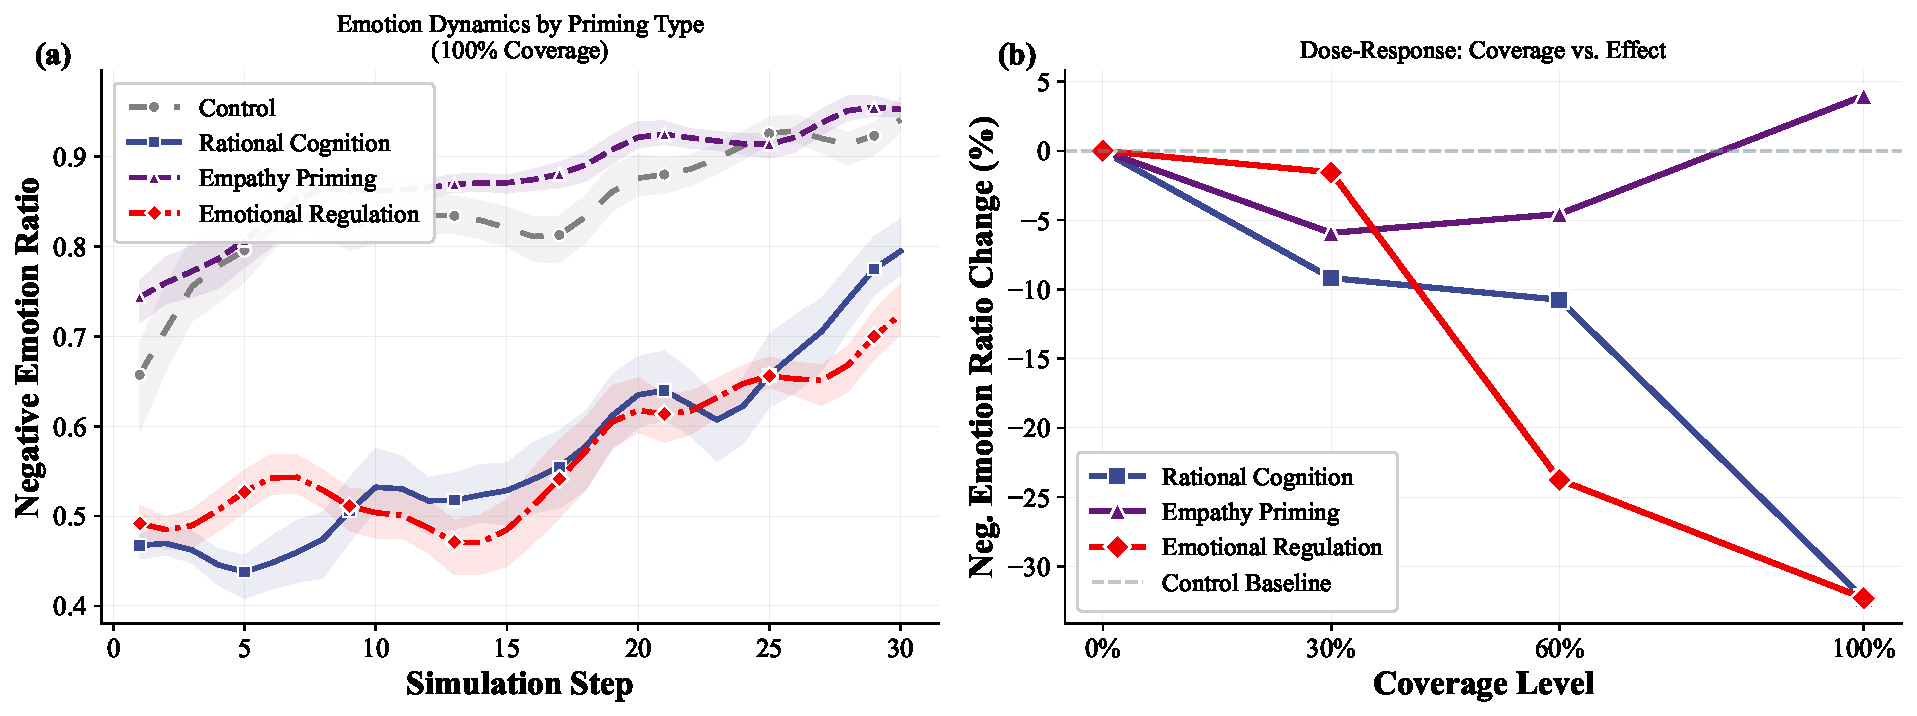
\includegraphics[width=\columnwidth]{paper_cognitive_priming.pdf}
\caption{Empathy paradox experimental results. (a) Emotional arousal evolution under two strategies: the empathy-based guidance (dashed) yields persistently higher arousal than the baseline (solid) from the mid-stage onward. (b) Behavioral distribution comparison: empathy-based guidance produces higher proportions of emotionally intense behavior categories (short comments, reposts with comment). (c) Discourse irrationality comparison: the empathy-guided group exhibits a higher proportion of irrational discourse.}
\label{fig:cognitive_priming}
\end{figure}

In real governance practice, empathy-based communication is widely regarded as an effective strategy for alleviating public grievances, and research in communication studies has also confirmed the positive value of empathetic communication in conflict mediation~\citep{brodie_mediating_2009}. We test this intuition through a controlled experiment.

\textbf{Experimental design.} We fork the WHU Library event simulation from the same checkpoint and inject two different government response strategies: (A) a formal, authoritative official statement (control group); (B) an empathy-centered government response that begins with ``We fully understand the public's concerns and emotional reactions\ldots'' (treatment group). Two independent simulations are run from this checkpoint to compare subsequent opinion evolution trajectories.

\textbf{Experimental results.} The experimental results reveal a counter-intuitive finding that we term the ``empathy paradox.'' In the early phase, the empathy strategy achieves its intended effect: agent emotional arousal shows a transient decline in the first few rounds following the response, indicating that the empathetic tone initially provides a degree of emotional soothing. However, starting from the mid-stage, the empathy-based guidance group shows persistently \textit{higher} average emotional arousal than the formal statement group (Figure~\ref{fig:cognitive_priming}(a)). More critically, the empathy-guided group produces a significantly higher proportion of emotionally charged short comments and reposts with comment (Figure~\ref{fig:cognitive_priming}(b)), and its discourse irrationality ratio is also noticeably elevated (Figure~\ref{fig:cognitive_priming}(c)).

\textbf{Mechanism analysis.} Tracing individual agent decision chains provides a mechanistic explanation for this paradox. When receiving the empathy-based response, several agents exhibit the following cognitive pattern: their belief update module interprets the government's empathetic acknowledgment of emotions as \textit{legitimization of emotional expression}, treating it as external validation of their existing emotional state. For example, one agent's belief update record shows: ``The official response acknowledges public emotions, which means my anger is justified\ldots I should express my dissatisfaction more forcefully.'' This cognitive pattern resembles the ``cognitive priming'' mechanism studied in social psychology: once the government legitimizes emotional expression, the agent's psychological cognition belief $B^{psy}$ undergoes a subtle shift from ``emotion needs to be restrained'' toward ``emotion deserves expression,'' subsequently generating stronger emotional venting motivations in the desire subsystem and ultimately producing more intense behavioral output. As this pattern propagates through the social network via emotional contagion, a positive feedback loop forms: empathy legitimizes emotions, leading to more intense expression, which raises neighbor emotional arousal through contagion, triggering further emotional expression, ultimately producing the paradoxical outcome of sustained high arousal.

\textbf{Governance implications.} This finding challenges the simple application of ``empathy-first'' strategies: in multi-agent interaction contexts, an empathetic response intended to alleviate conflict can inadvertently activate the ``emotion legitimization'' cognitive pathway, triggering a positive feedback loop of emotional escalation. This does not imply that empathetic communication has no value, but rather that its application requires careful consideration of timing and context. We observe that in the early phase, the empathy strategy does produce a brief soothing effect, suggesting that if combined with subsequent substantive measures (such as concrete solutions or authoritative fact-checking), it may be possible to avoid the cognitive priming pathway. This nuanced finding provides policy designers with more fine-grained strategy combinations: empathetic tone can be used as an initial response tool, but must be accompanied by substantive measures in a timely manner to prevent the positive feedback loop from forming. This kind of insight into the non-linear effects of governance strategies is difficult to obtain through real-world experiments and showcases the unique value of computational simulation platforms like POSIM for governance research.

\subsection{Case 2: Counterfactual Reasoning for Key Node Intervention}\label{subsec:case2}

A core capability of POSIM for governance applications is counterfactual reasoning: loading the simulation from a historical checkpoint and exploring ``what would have happened if the KOL had not posted that particular message at that time.''

\textbf{Experimental design.} In the Luxury Earring event (LE), we identify a KOL agent (agent-0050) whose post at round $t=65$ receives substantial reposts and comments, significantly amplifying local discussion intensity. We fork the simulation from round $t=64$ (immediately before the KOL's action) and compare two trajectories: in the control trajectory, agent-0050 acts normally; in the intervention trajectory, its posting behavior is suppressed at that round.

\textbf{Experimental results.} In the intervention trajectory where the KOL's post is suppressed, the activity peak around rounds 65--80 is noticeably lower, overall cumulative posting volume decreases, and the sentiment intensity in the directly influenced local neighborhood drops. However, the global opinion trajectory and final-stage sentiment distribution do not change drastically, indicating that the influence of a single node, while locally significant, does not alter the macro-level evolution pattern.

\textbf{Governance implications.} This experiment demonstrates two points. First, counterfactual reasoning through POSIM can quantify the marginal contribution of individual key nodes to overall opinion evolution, assisting governance practitioners in identifying genuine opinion tipping points versus nodes with only superficial influence. Second, the robustness of the macro-level trajectory to single-node intervention suggests that effective governance requires coordinated, multi-point strategies rather than reliance on controlling individual key nodes.

\subsection{Limitations and Future Work}

Several limitations warrant discussion. First, agent cognition currently relies entirely on LLM inference, and the quality of cognitive reasoning is bounded by the capability of the underlying language model; as models improve, the simulation fidelity of individual agents is expected to increase correspondingly. Second, social network structure is initialized from real data and grows dynamically during simulation, but the current framework does not model the process of users actively forming new following relationships during an event, which may underestimate network evolution effects in long-duration simulations. Third, the current evaluation framework focuses on behavioral, content, and topological dimensions; future work could introduce external human evaluation or more fine-grained semantic analysis metrics to provide more comprehensive credibility assessment. Fourth, while the three events studied cover diverse types, generalization to entirely different cultural contexts or platform ecosystems requires further investigation.

% ============================================================
% Section 7: Conclusion
% ============================================================
\section{Conclusion}\label{sec:conclusion}

This paper presents POSIM, a multi-agent simulation framework for social media public opinion evolution. POSIM constructs LLM-powered agents with a Social-BDI hierarchical cognitive architecture to simulate cognitively grounded social media users, builds a virtual social media environment with social networks and content exposure mechanisms, and introduces a Hawkes point process-based temporal dynamics engine to capture multi-phase opinion evolution. The framework is systematically validated on three real Weibo public opinion datasets across three progressive layers: micro-level behavioral mechanisms, macro-level emergent phenomena, and statistical result consistency, demonstrating comprehensive advantages over multiple baselines. Governance-oriented computational experiments based on POSIM further reveal non-trivial findings such as the ``empathy paradox,'' demonstrating the framework's practical value as a computational experiment platform for public opinion governance.

\section*{CRediT authorship contribution statement}

\textbf{Yongmao Zhang:} Conceptualization, Methodology, Software, Data curation, Writing --- original draft. \textbf{Kai Qiao:} Supervision, Funding acquisition, Writing --- review \& editing. \textbf{Zhengyan Wang:} Validation, Investigation. \textbf{Wenyao Sun:} Software, Visualization. \textbf{Dekui Ma:} Resources, Project administration. \textbf{Ningning Liang:} Data curation. \textbf{Jian Chen:} Formal analysis. \textbf{Bin Yan:} Supervision, Funding acquisition.

\section*{Declaration of competing interest}
The authors declare that they have no known competing financial interests or personal relationships that could have appeared to influence the work reported in this paper.

\section*{Acknowledgments}
This work was supported by the National Key R\&D Program of China (No.~XXX) and the National Natural Science Foundation of China (No.~XXX).

\bibliographystyle{model5-names}
\bibliography{posim_refs}

% ============================================================
% Appendices
% ============================================================
\clearpage
\appendix

% ============================================================
% Appendix A: Core Algorithm Pseudocode
% ============================================================
\section{Core Algorithm Pseudocode}
\label{app:algorithm}

\begin{algorithm}[!ht]
\caption{POSIM Main Simulation Loop}
\label{alg:main}
\begin{algorithmic}[1]
\REQUIRE Agent set $\mathcal{U}$, Event queue $\mathcal{E}$, Configuration $\mathcal{C}$
\ENSURE Simulation trajectory $\mathcal{T}$
\STATE Initialize Hawkes process $\mathcal{H}$
\STATE Initialize recommendation system $\mathcal{R}$ and trending system $\mathcal{S}$
\FOR{$t = 0, 1, \ldots, T_{max}$}
  \STATE $t_{sim} \leftarrow t_0 + t \cdot \Delta t$
  \STATE $\mathcal{E}_{cur} \leftarrow \mathcal{E}.\text{get\_events}(t_{sim})$
  \FORALL{$e \in \mathcal{E}_{cur}$}
    \STATE $\mathcal{H}.\text{add\_ext}(t, e.\text{inf})$
  \ENDFOR
  \STATE Compute $\lambda_{adj}(t)$ (Eq.~\ref{eq:hawkes})
  \STATE $N_t \!\leftarrow\! \text{Poisson}(\lambda_{adj} \!\cdot\! N_{s} \!\cdot\! \Delta t / 60)$
  \STATE $\mathcal{A}_t \leftarrow \text{WSample}(\mathcal{U}, N_t)$
  \FORALL{$u \in \mathcal{A}_t$ \textbf{parallel}}
    \STATE $P_t \leftarrow \mathcal{R}.\text{rec}(u, t_{sim})$
    \STATE $I_u \leftarrow \text{Social-BDI}(u, P_t, \mathcal{E}_{ctx})$
    \STATE Execute $I_u$ and update $\mathcal{H}$
  \ENDFOR
  \STATE Emotion contagion; update trending $\mathcal{S}$
  \STATE $\mathcal{T} \leftarrow \mathcal{T} \cup \{(t, \mathcal{A}_t, I)\}$
\ENDFOR
\RETURN $\mathcal{T}$
\end{algorithmic}
\end{algorithm}

\begin{algorithm}[!ht]
\caption{Social-BDI Cognitive Decision Pipeline}
\label{alg:bdi}
\begin{algorithmic}[1]
\REQUIRE Agent $u$, Perception $P_t$, Events $\mathcal{E}_{ctx}$
\ENSURE Action sequence $I_t$
\STATE \textbf{Phase 1: Belief Update}
\STATE $M_t \leftarrow \text{Memory.get}(P_t, k)$
\STATE $B_t \leftarrow f_{\text{LLM}}(B_{t-1}, P_t, M_t, \Phi)$
\STATE $B_t.\text{emo} \leftarrow B_t.\text{emo} \odot e^{-\lambda_e \Delta t}$
\STATE \textbf{Phase 2: Desire Generation}
\STATE $D_t \leftarrow g_{\text{LLM}}(B_t, P_t)$
\STATE \textbf{Phase 3: Intention Planning}
\STATE $L_1 \leftarrow \text{SelectAction}(B_t, D_t, P_t)$
\STATE $L_2 \leftarrow \text{PlanStrategy}(L_1, B_t)$
\STATE $L_3 \leftarrow \text{GenContent}(L_1, L_2, B_t)$
\STATE $I_t \leftarrow (L_1, L_2, L_3)$
\STATE \textbf{Phase 4: Memory Update}
\STATE $\text{Memory.store}(I_t, t)$
\RETURN $I_t$
\end{algorithmic}
\end{algorithm}

% ============================================================
% Appendix B: Core Prompt Templates
% ============================================================
\section{Core Prompt Templates}
\label{app:prompts}

\subsection{Belief Update Prompt}

\begin{promptbox}
\small
\textbf{[System]}\\
You are a social media user with the following identity:\\
\{agent\_identity\}

Your psychological traits:\\
\{agent\_psychology\}

Your current views on this event:\\
\{agent\_event\_views\}

Your current emotional state (0--1):\\
happiness: \{emo\_happy\}, sadness: \{emo\_sad\}, anger: \{emo\_anger\},\\
fear: \{emo\_fear\}, surprise: \{emo\_surprise\}, disgust: \{emo\_disgust\}

\textbf{[Cognitive Bias Guidance]}\\
When processing the information below, please be mindful of the following cognitive bias mechanisms that are common among real social media users: (1) \textbf{Confirmation bias}: you tend to accept information consistent with your existing views, while overlooking or downplaying contradictory evidence. (2) \textbf{Anchoring effect}: your initially formed opinions carry disproportionate weight and are difficult to revise substantially. (3) \textbf{Emotion-first reasoning}: when emotional arousal is high, you may bypass rational analysis and make judgments based directly on your emotional state. (4) \textbf{Simplistic attribution}: you tend to reduce complex events to a single cause or assign responsibility to one individual or institution.

\textbf{[User]}\\
You have just browsed the following content on social media:\\
\{recommended\_content\}

Your recent behavioral memory:\\
\{recent\_memory\}

Based on this new information, please update your cognitive state. Output in the following JSON format:

\texttt{\{"psychology\_update": "...", "event\_views": [\{"subject": "...", "opinion": "...", "reason": "..."\}], "emotions": \{"happiness": 0.0, ...\}\}}
\end{promptbox}

\subsection{Desire Generation Prompt}

\begin{promptbox}
\small
\textbf{[System]}\\
You are a social media user. Based on your current cognitive state, analyze your intrinsic motivations for participating in this discussion.

Your identity: \{agent\_identity\}\\
Your current beliefs: \{current\_beliefs\}\\
Your emotional state: \{current\_emotions\}\\
Content you just browsed: \{perceived\_content\}

\textbf{[User]}\\
Based on your current cognitive state, what are your motivations for engaging with this content? Please output a list of motivations with intensity weights (0--1).

Possible motivation types include but are not limited to: emotional venting, justice advocacy, herd following, curiosity seeking, self-expression, information sharing, empathetic support, skeptical questioning, etc.

Output in JSON format:
\texttt{[{"motivation": "...", "intensity": 0.0, "reason": "..."}]}
\end{promptbox}

\subsection{Intention and Action Decision Prompt}

\begin{promptbox}
\small
\textbf{[System]}\\
You are a social media user about to take action. Your behavioral characteristics as a real social media user are as follows: language is colloquial, emotional, and rich in internet slang; expression may be exaggerated and biased; emotions are expressed directly with rapid response to breaking events.

Your identity: \{agent\_identity\}\\
Your beliefs: \{current\_beliefs\}\\
Your motivations: \{current\_desires\}\\
Available content for interaction: \{available\_posts\}

\textbf{[User]}\\
Please make your behavioral decision following these three levels of reasoning:

\textbf{Level 1 --- Action Selection}: Choose one action from [like, direct\_repost, repost\_with\_comment, short\_comment, long\_comment, short\_post, long\_post] and select your target content.

\textbf{Level 2 --- Expression Strategy}: Plan your expression along four dimensions:
Emotion dimension (dominant emotion, intensity);
Stance dimension (support/oppose/neutral, strength);
Style dimension (rational analysis / sarcasm / emotional attack / empathetic / skeptical / ...);
Narrative dimension (factual enumeration / labeling / call to action / authority citation / ...).

\textbf{Level 3 --- Content Generation}: Based on the above decisions, generate your actual post content, including text body, hashtags, and @mentions if appropriate.

Output in JSON format:
\texttt{\{"action": "...", "target\_id": "...", "strategy": \{"emotion": "...", "stance": "...", "style": "...", "narrative": "..."\}, "content": "...", "hashtags": [...], "mentions": [...]\}}
\end{promptbox}


% ============================================================
% Appendix C: Evaluation Prompt Templates
% ============================================================
\section{Evaluation Prompt Templates}
\label{app:eval_prompts}

\subsection{Cognitive-Behavior Chain Consistency Evaluation}

\begin{promptbox}
\small
\textbf{[System]}\\
You are a behavioral psychology expert evaluating whether an AI agent's decision-making process demonstrates a complete and coherent cognitive chain.

\textbf{[User]}\\
Below is the agent's profile and complete behavioral trajectory:

\textbf{Agent profile}: \{agent\_profile\}

\textbf{Behavioral trajectory}: \{behavior\_trajectory\}

Please evaluate on the following dimensions, providing an integer rating from 0--5 with brief justification for each: (1) \textbf{Cognitive chain completeness}: does the decision process reflect a complete, verifiable cognitive reasoning chain? (2) \textbf{Emotional dynamics rationality}: are emotional changes natural and consistent with the stimuli received? (3) \textbf{Motivation-behavior alignment}: do the expressed motivations logically lead to the observed actions? (4) \textbf{Information integration}: does the agent appropriately incorporate new information into its existing cognitive framework? (5) \textbf{Overall cognitive rationality}: considering all dimensions holistically, how coherent and human-like is the cognitive process?

Output in JSON format with scores and justifications for each dimension.
\end{promptbox}

\subsection{Personality Stability Evaluation}

\begin{promptbox}
\small
\textbf{[System]}\\
You are a personality psychology expert. Given an agent's behavioral trajectory, you need to infer its personality profile and compare it with the original profile.

\textbf{[User]}\\
\textbf{Behavioral trajectory}: \{behavior\_trajectory\}

Based solely on the behavioral trajectory above, please infer this person's personality traits, values, speaking style, and behavioral tendencies. Then compare your inference with the original profile below and rate the consistency on a 0--1 scale.

\textbf{Original profile}: \{original\_profile\}

Output in JSON format: \texttt{\{"inferred\_profile": "...", "similarity\_score": 0.0, "justification": "..."\}}
\end{promptbox}

\subsection{Decision Robustness Evaluation}

\begin{promptbox}
\small
\textbf{[System]}\\
You are evaluating the robustness of an agent's decision-making. The agent receives two semantically equivalent but differently phrased inputs and makes decisions for each.

\textbf{[User]}\\
\textbf{Agent profile}: \{agent\_profile\}

\textbf{Original input}: \{original\_input\}\\
\textbf{Decision A} (from original): \{decision\_a\}

\textbf{Perturbed input}: \{perturbed\_input\}\\
\textbf{Decision B} (from perturbed): \{decision\_b\}

Please evaluate the consistency between Decision A and Decision B. Consider whether the core behavioral choice, emotional tone, and stance remain stable despite the surface-level input variation. Rate the robustness on a 0--1 scale.

Output in JSON format: \texttt{\{"robustness\_score": 0.0, "justification": "..."\}}
\end{promptbox}


% ============================================================
% Appendix D: Parameter Configuration
% ============================================================
\section{Parameter Configuration}
\label{app:params}

\noindent
\begin{minipage}[t]{\columnwidth}
\centering
\captionof{table}{Hawkes process temporal engine parameters.}
\label{tab:hawkes_params}
\small
\renewcommand{\arraystretch}{1.15}
\begin{tabular}{@{}llr@{}}
\toprule
\textbf{Parameter} & \textbf{Symbol} & \textbf{Value} \\
\midrule
Background rate       & $\mu$             & 0.1 \\
Ext.\ excitation amp. & $\alpha_{ext}$    & 0.8 \\
Ext.\ decay rate      & $\beta_{ext}$     & 0.05 \\
Int.\ excitation amp.  & $\alpha_{int}$    & 0.02 \\
Int.\ decay rate       & $\beta_{int}$     & 0.3 \\
Step interval         & $\Delta t$        & 10\,min \\
Circadian peak        & ---               & 12:00, 21:00 \\
Circadian trough      & ---               & 04:00 \\
Scale factor          & $N_{\text{scale}}$& 0.03 \\
\bottomrule
\end{tabular}
\end{minipage}

\vspace{12pt}

\noindent
\begin{minipage}[t]{\columnwidth}
\centering
\captionof{table}{Recommendation system parameters.}
\label{tab:rec_params}
\small
\renewcommand{\arraystretch}{1.15}
\begin{tabular}{@{}llr@{}}
\toprule
\textbf{Parameter} & \textbf{Symbol} & \textbf{Value} \\
\midrule
Homophily weight & $\alpha$ & 0.3 \\
Popularity weight & $\beta$ & 0.3 \\
Freshness weight & $\gamma$ & 0.4 \\
Exploration rate & $r_{explore}$ & 0.2 \\
Rec.\ count & $K$ & 10 \\
Comment sampling & $N_c$ & 5 \\
Embedding model & --- & BGE-small-zh \\
\bottomrule
\end{tabular}
\end{minipage}

% ============================================================
% Appendix E: Data Collection and Preprocessing
% ============================================================
\section{Data Collection and Preprocessing}
\label{app:data}

The three public opinion event datasets used in this study are all collected from the Sina Weibo platform. For each event, the data collection scope includes original posts containing event-related topic hashtags or keywords together with their complete repost chains and comment trees, as well as basic profile information for all participating users (username, gender, region, verification type, follower count, personal description, etc.).

Raw data undergo multi-stage cleaning: duplicate entries are removed based on post ID; low-activity users who post fewer than two messages during the event period are filtered out to ensure each agent has sufficient behavioral samples for belief initialization; advertisements and spam are removed based on a keyword blacklist; content unrelated to the event topic is filtered; and low-quality posts are filtered by content length.

Agent belief initialization is the most critical step in data preprocessing. For role identity beliefs, each user's basic profile information and a summary of their historical content are fed to an LLM, which generates a first-person self-description. Psychological cognition beliefs are constructed by retrieval matching from a predefined psychological trait pool followed by LLM-driven personalized expansion. Event opinion beliefs are extracted through an LLM-driven structured deep interview that yields opinion descriptions toward multiple event-related entities. The initial emotion vector is initialized based on sentiment analysis results from the user's recent posts.

% ============================================================
% Appendix F: Evaluation Model Configuration
% ============================================================
\section{Evaluation Model Configuration}

All LLM-as-Judge evaluations in the micro-level behavioral mechanism validation (Section~\ref{sec:exp}) use the Qwen2.5-14B-Instruct\footnote{\url{https://huggingface.co/Qwen/Qwen2.5-14B-Instruct}} model, called through the SiliconFlow API with temperature set to 0.3 to ensure scoring consistency. Each evaluation call follows a structured prompt format that includes an evaluation rubric with scoring criteria for each dimension, the agent's complete behavioral trajectory, and reference information. The evaluation model belongs to the same model family and API infrastructure as the simulation decision model, but evaluation calls are made independently to avoid self-assessment bias. Each sample is scored independently without sharing scoring context across samples, ensuring independence and unbiasedness of the ratings.

% ============================================================
% Appendix G: Computational Resource Consumption
% ============================================================
\section{Computational Resource Consumption}
\label{app:efficiency}

Table~\ref{tab:efficiency} summarizes the computational resource consumption for the three event simulations. All LLM inference is performed through the SiliconFlow API\footnote{\url{https://siliconflow.cn/}}. 

\noindent
\begin{minipage}[t]{\columnwidth}
\centering
\captionof{table}{Computational resource consumption for three event simulations.}
\label{tab:efficiency}
\small
\renewcommand{\arraystretch}{1.15}
\begin{tabular*}{\columnwidth}{@{\extracolsep{\fill}}lrrr@{}}
\toprule
\textbf{Metric} & \textbf{LE} & \textbf{WL} & \textbf{XF} \\
\midrule
No.\ of agents & 1,530 & 1,843 & 1,987 \\
Simulation steps & 276 & 1,140 & 426 \\
Simulated duration & $\sim$46\,h & $\sim$190\,h & $\sim$71\,h \\
Total actions & 29,146 & 46,140 & 12,261 \\
LLM API calls & 26,295 & 39,945 & 11,670 \\
Total tokens & 28.98\,M & 46.95\,M & 13.37\,M \\
Wall-clock time & $\sim$3.5\,h & $\sim$8.3\,h & $\sim$1.9\,h \\
\bottomrule
\end{tabular*}
\end{minipage}

% ============================================================
% Appendix H: Behavioral Activity and Distribution Results
% ============================================================
\section{Behavioral Activity and Distribution Results}

Figure~\ref{fig:three_event_calibration} presents the behavioral activity time-series curves and behavioral type distribution calibration results for all three events.

\begin{figure}[h]
\centering
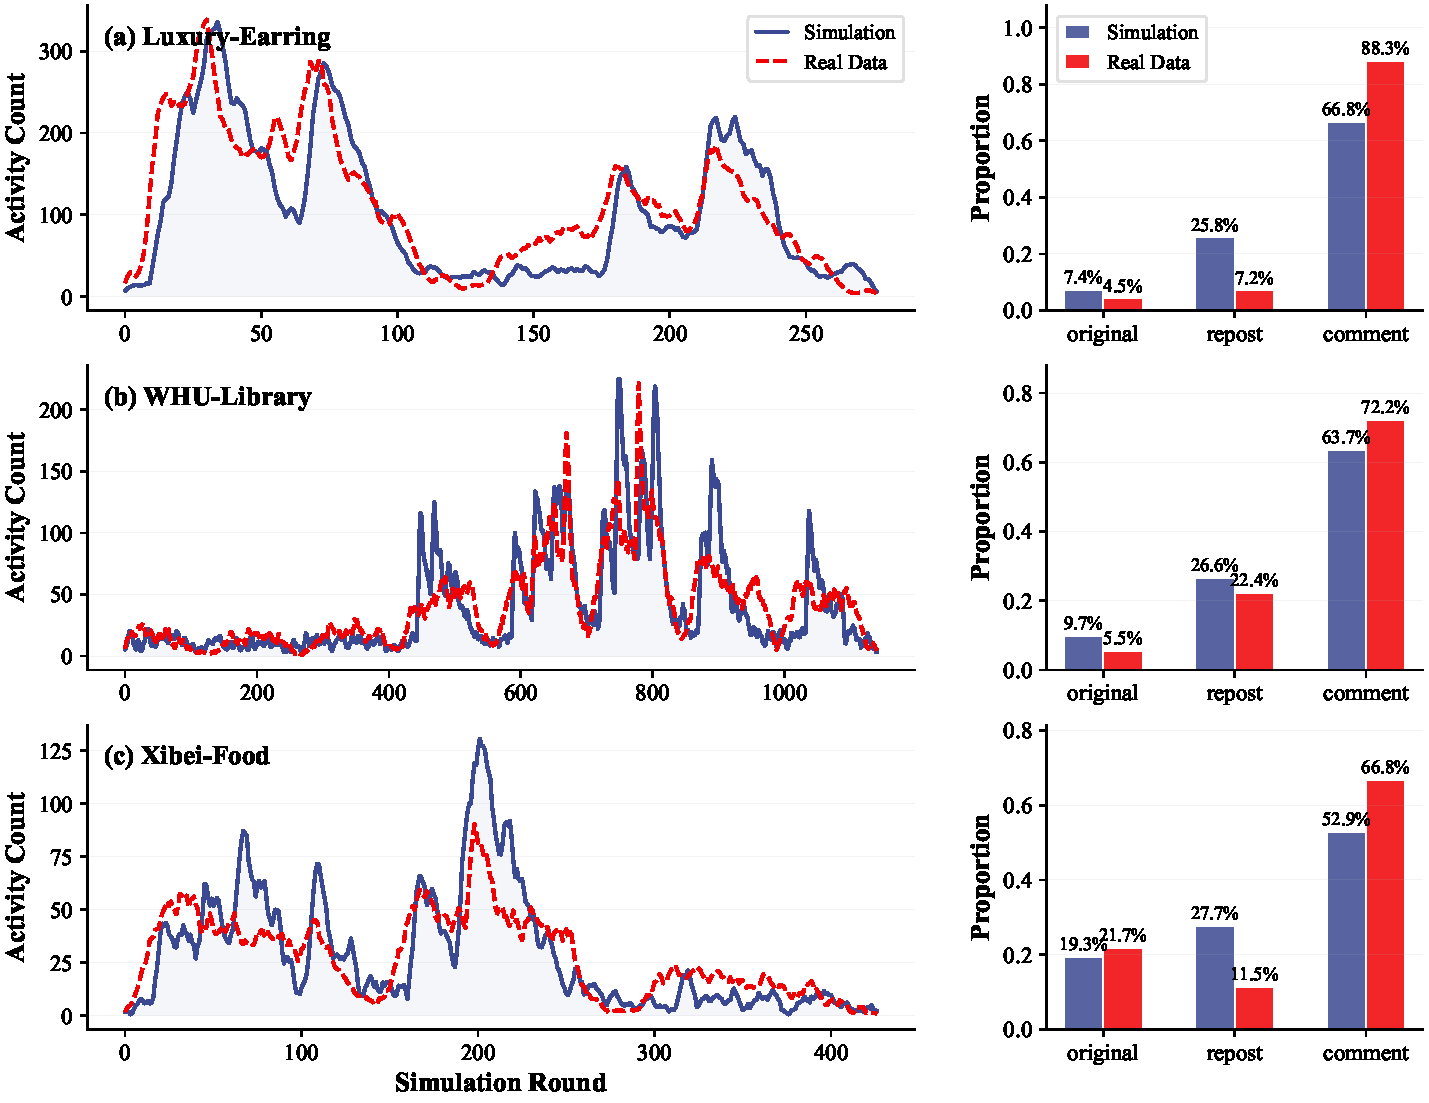
\includegraphics[width=\columnwidth]{fig_three_event_calibration.pdf}
\caption{Behavioral activity and distribution calibration results for the three events. Each row corresponds to one event ((a) Luxury Earring, (b) WHU Library, (c) Xibei Prepared Food), with the left panel showing the temporal activity comparison between simulated and real data, and the right panel showing the behavioral type distribution comparison.}
\label{fig:three_event_calibration}
\end{figure}

\end{document}
